\documentclass[a4paper,12pt]{article}
\usepackage{amsmath}
\usepackage{amssymb,amsthm,graphicx}
\usepackage{enumitem}
\usepackage{color}
\usepackage{epsfig}
%\usepackage{graphics}
\usepackage{graphicx}
\usepackage{pdfpages}
\usepackage[font=small]{caption}
\usepackage[hang,flushmargin]{footmisc} 
\usepackage{float}
\usepackage{booktabs}
\usepackage[mathscr]{euscript}
\usepackage{natbib}
\usepackage{setspace}
\usepackage{mathrsfs}
\usepackage[left=2.8cm,right=2.8cm,bottom=2.8cm,top=2.8cm]{geometry}
\parindent0pt 


% General

\newcommand{\reals}{\mathbb{R}}
\newcommand{\integers}{\mathbb{Z}}
\newcommand{\naturals}{\mathbb{N}}

\newcommand{\pr}{\mathbb{P}}        % probability
\newcommand{\ex}{\mathbb{E}}        % expectation
\newcommand{\var}{\textnormal{Var}} % variance
\newcommand{\cov}{\textnormal{Cov}} % covariance

\newcommand{\law}{\mathcal{L}} % law of X
\newcommand{\normal}{N}        % normal distribution 

\newcommand{\argmax}{\textnormal{argmax}}
\newcommand{\argmin}{\textnormal{argmin}}

\newcommand{\ind}{\mathbbm{1}} % indicator function
\newcommand{\kernel}{K} % kernel function
\newcommand{\wght}{W} % kernel weight
\newcommand{\thres}{\pi} % threshold parameter


% Convergence

\newcommand{\convd}{\stackrel{d}{\longrightarrow}}              % convergence in distribution
\newcommand{\convp}{\stackrel{P}{\longrightarrow}}              % convergence in probability
\newcommand{\convas}{\stackrel{\textrm{a.s.}}{\longrightarrow}} % convergence almost surely
\newcommand{\convw}{\rightsquigarrow}                           % weak convergence


% Theorem-like declarations

\theoremstyle{plain}

\newtheorem{theorem}{Theorem}[section]
\newtheorem{prop}[theorem]{Proposition}
\newtheorem{lemma}[theorem]{Lemma}
\newtheorem{corollary}[theorem]{Corollary}
\newtheorem*{theo}{Theorem}
\newtheorem{propA}{Proposition}[section]
\newtheorem{lemmaA}[propA]{Lemma}
\newtheorem{definition}{Definition}[section]
\newtheorem{remark}{Remark}[section]
\renewcommand{\thelemmaA}{A.\arabic{lemmaA}}
\renewcommand{\thepropA}{A.\arabic{propA}}
\newtheorem*{algo}{Clustering Algorithm}


% Theorem numbering to the left

\makeatletter
\newcommand{\lefteqno}{\let\veqno\@@leqno}
\makeatother


% Heading

\newcommand{\heading}[2]
{  \setcounter{page}{1}
   \begin{center}

   \phantom{Distance to upper boundary}
   \vspace{0.5cm}

   {\LARGE \textbf{#1}}
   \vspace{0.4cm}
 
   {\LARGE \textbf{#2}}
   \end{center}
}


% Authors

\newcommand{\authors}[4]
{  \parindent0pt
   \begin{center}
      \begin{minipage}[c][2cm][c]{5cm}
      \begin{center} 
      {\large #1} 
      \vspace{0.05cm}
      
      #2 
      \end{center}
      \end{minipage}
      \begin{minipage}[c][2cm][c]{5cm}
      \begin{center} 
      {\large #3}
      \vspace{0.05cm}

      #4 
      \end{center}
      \end{minipage}
   \end{center}
}

%\newcommand{\authors}[2]
%{  \parindent0pt
%   \begin{center}
%   {\large #1} 
%   \vspace{0.1cm}
%      
%   #2 
%   \end{center}  
%}


% Version

\newcommand{\version}[1]
{  \begin{center}
   {\large #1}
   \end{center}
   \vspace{3pt}
} 







\renewcommand{\baselinestretch}{1.2}
\numberwithin{equation}{section}
\allowdisplaybreaks[1]




\begin{document}



\begin{center}
{\LARGE \textbf{Multiscale Inference for}} \\[0.35cm]
{\LARGE \textbf{Nonparametric Time Trends}}
\end{center}



\section{The model}\label{sec-model}


The actual model setting for the test problems considered in Sections \ref{sec-method} and \ref{sec-test-shape} is as follows: We observe a time series $\{Y_t: 1 \le t \le T \}$ of length $T$ which satisfies the model equation 
\begin{equation}\label{model1}
Y_t = m \Big( \frac{t}{T} \Big) + \varepsilon_t 
\end{equation}
for $1 \le t \le T$. Here, $m$ is an unknown nonparametric regression function defined on $[0,1]$ and $\{ \varepsilon_t: 1 \le t \le T \}$ is a zero-mean stationary error process. For simplicity, we restrict attention to equidistant design points $x_t = t/T$. However, our methods and theory can also be carried over to non-equidistant designs. The stationary error process $\{\varepsilon_t\}$ is assumed to have the following properties: 
\begin{enumerate}[label=(C\arabic*),leftmargin=1.05cm]

\item \label{C-err1} The variables $\varepsilon_t$ allow for the representation $\varepsilon_t = G(\ldots,\eta_{t-1},\eta_t,\eta_{t+1},\ldots)$, where $\eta_t$ are i.i.d.\ random variables and $G: \reals^\integers \rightarrow \reals$ is a measurable function. 

\item \label{C-err2} It holds that $\| \varepsilon_t \|_q < \infty$ for some $q > 4$, where $\| \varepsilon_t \|_q = (\ex|\varepsilon_t|^q)^{1/q}$. 

\end{enumerate}
Following \cite{Wu2005}, we impose conditions on the dependence structure of the error process $\{\varepsilon_t\}$ in terms of the physical dependence measure $d_{t,q} = \| \varepsilon_t - \varepsilon_t^\prime \|_q$, where $\varepsilon_t^\prime = G(\ldots,\eta_{-1},\eta_0^\prime,\eta_1,\ldots,\eta_{t-1},\eta_t,\eta_{t+1},\ldots)$ with $\{\eta_t^\prime\}$ being an i.i.d.\ copy of $\{\eta_t\}$. In particular, we assume the following: 
\begin{enumerate}[label=(C\arabic*),leftmargin=1.05cm]
\setcounter{enumi}{2}

\item \label{C-err3} Define $\Theta_{t,q} = \sum\nolimits_{|s| \ge t} d_{s,q}$ for $t \ge 0$. It holds that 
\[ \Theta_{t,q} = O \big( t^{-\tau_q} (\log t)^{-A} \big), \]
where
\[ \tau_q = \frac{q^2 - 4 + (q-2) \sqrt{q^2 + 20q + 4}}{8q} \]
and $A > \frac{2}{3} (1/q + 1 + \tau_q)$. 

\end{enumerate}
The conditions \ref{C-err1}--\ref{C-err3} are fulfilled by a wide range of stationary processes $\{\varepsilon_t\}$. As a first example, consider linear processes of the form $\varepsilon_t = \sum\nolimits_{i=0}^{\infty} c_i \eta_{t-i}$ with $\| \varepsilon_t \|_q < \infty$, where $c_i$ are absolutely summable coefficients and $\eta_t$ are i.i.d.\ innovations with $\ex[\eta_t] = 0$ and $\| \eta_t\|_q < \infty$. Trivially, \ref{C-err1} and \ref{C-err2} are fulfilled in this case. Moreover, if $|c_i| = O(\rho^i)$ for some $\rho \in (0,1)$, then \ref{C-err3} is easily seen to be satisfied as well. As a special case, consider an ARMA process $\{\varepsilon_t\}$ of the form $\varepsilon_t + \sum\nolimits_{i=1}^p a_i \varepsilon_{t-i} = \eta_t + \sum\nolimits_{j=1}^r b_j \eta_{t-j}$  with $\| \varepsilon_t \|_q < \infty$, where $a_1,\ldots,a_p$ and $b_1,\ldots,b_r$ are real-valued parameters. As before, we let $\eta_t$ be i.i.d.\ innovations with $\ex[\eta_t] = 0$ and $\| \eta_t\|_q < \infty$. Moreover, we suppose that the complex polynomials $A(z) = 1 + \sum\nolimits_{j=1}^p a_jz^j$ and $B(z) = 1 + \sum\nolimits_{j=1}^r b_jz^j$ do not have any roots in common. If $A(z)$ does not have any roots inside the unit disc, then the ARMA process $\{ \varepsilon_t \}$ is stationary and causal. Specifically, it has the representation $\varepsilon_t = \sum\nolimits_{i=0}^{\infty} c_i \eta_{t-i}$ with $|c_i| = O(\rho^i)$ for some $\rho \in (0,1)$, implying that \ref{C-err1}--\ref{C-err3} are fulfilled. The results in \cite{WuShao2004} show that condition \ref{C-err3} (as well as the other two conditions) is not only fulfilled for linear time series processes but also for a variety of non-linear processes. 


The model setting for the test problem analyzed in Section \ref{sec-test-equality} is closely related to the setting discussed above. The main difference is that we observe several rather than only one time series. In particular, we observe time series $\mathcal{Y}_i = \{Y_{it}: 1 \le t \le T \}$ of length $T$ for $1 \le i \le n$. Each time series $\mathcal{Y}_i$ satisfies the regression equation \begin{equation}\label{model2}
Y_{it} = m_i \Big( \frac{t}{T} \Big) + \alpha_i + \varepsilon_{it} 
\end{equation}
for $1 \le t \le T$, where $m_i$ is an unknown nonparametric function defined on $[0,1]$, $\alpha_i$ is a (deterministic or random) intercept term and $\mathcal{E}_i = \{ \varepsilon_{it}: 1 \le t \le T \}$ is a zero-mean stationary error process. For identification, we normalize the functions $m_i$ such that $\int_0^1 m_i(u) du = 0$ for all $1 \le i \le n$. The conditions on the error processes $\mathcal{E}_i$ can be summarized as follows: The processes $\mathcal{E}_i$ are independent across $i$ and each process $\mathcal{E}_i$ satisfies the conditions \ref{C-err1}--\ref{C-err3}. We thus work with essentially the same error structure as in the context of model \eqref{model1}. For simplicity, we assume throughout the paper that the number of time series $n$ in model \eqref{model2} is fixed. Note however that our theoretical results can be easily adapted to the case where $n$ slowly grows with the sample size $T$. 



\section{The multiscale method}\label{sec-method}


In this section, we introduce our multiscale test method and the underlying theory for the simple hypothesis $H_0: m = 0$ in model \eqref{model1}. Both the method and the theory for this simple case can be easily adapted to more interesting test problems as we will see in Sections \ref{sec-test-shape} and \ref{sec-test-equality}. 
%The discussion can be regarded as providing a blueprint of our multiscale methods and the underlying theory, which is ready to adapt to more advanced test problems. 


\subsection{Construction of the test statistic}\label{subsec-method-stat}


To construct a multiscale test statistic for the hypothesis $H_0: m = 0$ in model \eqref{model1}, we consider the kernel averages
\begin{equation*}
\widehat{\psi}_T(u,h) = \sum\limits_{t=1}^T w_{t,T}(u,h) Y_t, 
\end{equation*}
where $w_{t,T}(u,h)$ is a kernel weight with $u \in [0,1]$ and the bandwidth parameter $h$. We in particular set 
\begin{equation}\label{weights}
w_{t,T}(u,h) = \frac{1}{\|K\|_{u,h,T}} K\Big( \frac{u - \frac{t}{T}}{h} \Big) \, \quad \text{with} \quad \|K\|_{u,h,T} = \Big\{\sum\limits_{t=1}^T  K^2\Big( \frac{u - \frac{t}{T}}{h} \Big)\Big\}^{1/2}, 
\end{equation}
where $K$ is a kernel function with the following properties: 
\begin{enumerate}[label=(C\arabic*),leftmargin=1.05cm]
\setcounter{enumi}{3}
\item \label{C-ker} The kernel $K$ is non-negative, symmetric about zero and integrates to one. Moreover, it has compact support $[-1,1]$ and is Lipschitz continuous, that is, $|K(v) - K(w)| \le C |v-w|$ for any $v,w \in \reals$ and some constant $C > 0$. 
\end{enumerate} 
The kernel average $\widehat{\psi}_T(u,h)$ is a local average of the observations $Y_1,\ldots,Y_T$ which gives positive weight only to data points $Y_t$ with $t/T \in [u-h,u+h]$. Hence, only observations $Y_t$ with $t/T$ close to the location $u$ are taken into account, the amount of localization being determined by the bandwidth $h$. Notably, $\var(\widehat{\psi}_T(u,h)) = \sigma^2 + o(1)$ for any fixed location $u$ and any bandwidth $h$ with $h \rightarrow 0$ and $Th \rightarrow \infty$, where $\sigma^2 = \sum\nolimits_{\ell=-\infty}^{\infty} \gamma(\ell)$ with $\gamma(\ell) = \cov(\varepsilon_t, \varepsilon_{t+\ell})$ is the long-run variance of the error terms. This means that the statistics $\widehat{\psi}_T(u,h)$ have approximately the same variance across $u$ and $h$ for sufficiently large sample sizes $T$. In what follows, we mainly consider normalized versions $\widehat{\psi}_T(u,h)/\widehat{\sigma}$ of the kernel averages $\widehat{\psi}_T(u,h)$, where $\widehat{\sigma}^2$ is an estimator of the long-run error variance $\sigma^2$. The problem of estimating $\sigma^2$ is discussed in detail in Section \ref{sec-error-var}. For the time being, we suppose that $\widehat{\sigma}^2$ is an estimator with reasonable theoretical properties. In particular, we assume that $\widehat{\sigma}^2 = \sigma^2 + O_p(1/\sqrt{T})$. 


Our multiscale statistic combines the kernel averages $\widehat{\psi}_T(u,h)$ for a wide range of different locations $u$ and bandwidths or scales $h$. Specifically, it takes into account all points $(u,h) \in \mathcal{G}_T$, where $\mathcal{G}_T$ is some subset of 
\[ \mathcal{G} =  \big\{ (u,h): [u-h,u+h] \subseteq [0,1] \text{ with } u \in [0,1] \text{ and } h \in [h_{\min},h_{\max}] \big\} \]
with $h_{\min}$ and $h_{\max}$ denoting some minimal and maximal bandwidth value, respectively. For our theory to work, we require the following conditions to hold:
\begin{enumerate}[label=(C\arabic*),leftmargin=1.05cm]
\setcounter{enumi}{4}

\item \label{C-grid} $|\mathcal{G}_T| = O(T^\theta)$ for some arbitrarily large but fixed constant $\theta > 0$, where $|\mathcal{G}_T|$ denotes the cardinality of $\mathcal{G}_T$. 

\item \label{C-h} $h_{\min} \gg T^{(2-q)/q} \log T$, that is, $h_{\min} / \{ T^{(2-q)/q} \log T \} \rightarrow \infty$ with $q > 4$ defined in \ref{C-err2} and $h_{\max} \le 1/2$.

\end{enumerate}
According to \ref{C-grid}, the number of points $(u,h)$ in $\mathcal{G}_T$ should not grow faster than $T^\theta$ for some arbitrarily large but fixed $\theta > 0$. This is a fairly weak restriction as it allows the set $\mathcal{G}_T$ to be extremely large as compared to the sample size $T$. For example, we may work with the set 
\begin{align*}
\mathcal{G}_T = \big\{ & (u,h): [u-h,u+h] \subseteq [0,1] \text{ with } u = t/T \text{ for some } 1 \le t \le T \\ & \text{ and } h \in [h_{\min},h_{\max}] \text{ with } h = t/T \text{ for some } 1 \le t \le T  \big\},
\end{align*}
which contains more than enough points $(u,h)$ for most practical applications. Condition \ref{C-h} imposes some restrictions on the minimal and maximal bandwidths $h_{\min}$ and $h_{\max}$ used in our multiscale approach. These conditions are fairly weak, allowing us to choose the bandwidth window $[h_{\min},h_{\max}]$ extremely large. In particular, we can choose the minimal bandwidth $h_{\min}$ to be of the order $T^{-1/2}$ for any $q > 4$, which means that we can let $h_{\min}$ converge to $0$ very quickly. Moreover, the maximal bandwidth $h_{\max}$ need not even converge to $0$, which implies that we can pick it very large.


%Our multiscale approach simultaneously takes into account a wide range of different locations $u$ and bandwidths or scales $h$, namely the points $(u,h)$ contained in the set 
%\[ \mathcal{G}_T = \big\{ (u,h): [u-h,u+h] \subseteq [0,1] \text{ with } u \in \mathcal{U}_T, h \in \mathcal{H}_T \text{ and } h_{\min} \le h \le h_{\max} \big\}. \]
%Here, $h_{\min}$ and $h_{\max}$ denote some minimal and maximal bandwidth values which are discussed in more detail below. Moreover, 
%\begin{align*} 
%\mathcal{U}_T & = \big\{ u \in [0,1]: u = t/M_T \text{ for some } 1 \le t \le M_T \big\} \\
%\mathcal{H}_T & = \big\{ h \in [0,1/2]: h = t/M_T^\prime \text{ for some } 1 \le t \le M_T^\prime \big\},
%\end{align*}
%where $\{M_T\}$ and $\{M_T^\prime\}$ are any sequences with $M_T = O(T^\gamma)$ and $M_T^\prime = O(T^{\gamma})$ for some arbitrarily large but fixed constant $\gamma > 0$, that is, $M_T$ and $M_T^\prime$ are allowed to grow as any fixed order polynomial of $T$ but they should not grow as fast as the exponential of $T$. 


Following the approach in \cite{DuembgenSpokoiny2001}, we define our multiscale statistic as 
\[ \widehat{\Psi}_T = \max_{(u,h) \in \mathcal{G}_T} \Big\{ \Big|\frac{\widehat{\psi}_T(u,h)}{\widehat{\sigma}}\Big| - \lambda(h) \Big\}, \] 
where $\lambda(h) = \sqrt{2 \log \{ 1/(2h) \}}$. As suggested there, we thus do not simply aggregate the individual statistics $\widehat{\psi}_T(u,h)/\widehat{\sigma}$ by taking the supremum over all points $(u,h) \in \mathcal{G}_T$ as in the traditional approach. We rather subtract the additive correction term $\lambda(h)$ from the statistics that correspond to the bandwidth level $h$. To see the heuristic idea behind the additive correction $\lambda(h)$, consider for a moment the uncorrected statistic
\[ \widehat{\Psi}_{T,\text{uncorrected}} = \max_{(u,h) \in \mathcal{G}_T} \Big|\frac{\widehat{\psi}_T(u,h)}{\widehat{\sigma}}\Big|. \]
For simplicity, assume that the errors $\varepsilon_t$ are i.i.d.\ normally distributed and neglect the estimation error in $\widehat{\sigma}$, that is, set $\widehat{\sigma} = \sigma$. Moreover, suppose that the set $\mathcal{G}_T$ only consists of points $(u_k,h_\ell) = ((2k - 1)h_\ell,h_\ell)$ with $k = 1,\ldots,\lfloor 1/2h_\ell \rfloor$ and $\ell = 1,\ldots,L$. In this case, we can write
\[ \widehat{\Psi}_{T,\text{uncorrected}} = \max_{1 \le \ell \le L} \max_{1 \le k \le \lfloor 1/2h_\ell \rfloor} \Big|\frac{\widehat{\psi}_T(u_k,h_\ell)}{\sigma}\Big|. \]
Under our simplifying assumptions, the statistics $\widehat{\psi}_T(u_k,h_\ell)/\sigma$ with $k = 1,\ldots,\lfloor 1/2h_\ell \rfloor$ are independent and standard normal for any given bandwidth $h_\ell$. Since the maximum over $\lfloor 1/2h \rfloor$ independent standard normal random variables is $\lambda(h) + o_p(1)$ as $h \rightarrow 0$, we obtain that $\max_{k} \widehat{\psi}_T(x_k,h_\ell)/\sigma$ is approximately of size $\lambda(h_\ell)$ for small bandwidths $h_\ell$. As $\lambda(h) \rightarrow \infty$ for $h \rightarrow 0$, this implies that $\max_{k} \widehat{\psi}_T(x_k,h_\ell)/\sigma$ tends to be much larger in size for small than for large bandwidth values. As a result, the stochastic behaviour of the uncorrected statistic $\widehat{\Psi}_{T,\text{uncorrected}}$ tends to be dominated by the statistics $\widehat{\psi}_T(x_k,h_\ell)$ corresponding to small bandwidths $h_\ell$. The additively corrected statistic $\widehat{\Psi}_T$, in contrast, puts the statistics $\widehat{\psi}_T(x_k,h_\ell)$ corresponding to different bandwidth values $h_\ell$ on a more equal footing, thus counteracting the dominance of small bandwidth values. 


\subsection{The test procedure}\label{subsec-method-test}


In order to formulate a test for the hypothesis $H_0: m = 0$, we still need to specify a critical value. To do so, we define the statistic
\begin{equation}\label{Phi-statistic}
\Phi_T = \max_{(u,h) \in \mathcal{G}_T} \Big\{ \Big|\frac{\phi_T(u,h)}{\sigma}\Big| - \lambda(h) \Big\},
\end{equation} 
where
\[ \phi_T(u,h) = \sum\limits_{t=1}^T w_{t,T}(u,h) \, \sigma Z_t \]
and $Z_t$ are independent standard normal random variables. The statistic $\Phi_T$ can be regarded as a Gaussian version of the test statistic $\widehat{\Psi}_T$ under the null hypothesis $H_0$. Let $q_T(\alpha)$ be the $(1-\alpha)$-quantile of $\Phi_T$. Importantly, the quantile $q_T(\alpha)$ can be computed by Monte Carlo simulations and can thus be regarded as known. Our multiscale test of the hypothesis $H_0: m = 0$ is now defined as follows: For a given significance level $\alpha \in (0,1)$, we reject $H_0$ if $\widehat{\Psi}_T > q_T(\alpha)$. 


\subsection{Theoretical properties of the test}\label{subsec-method-theo}


In order to examine the theoretical properties of our multiscale test, we introduce the statistic 
\begin{align}
\widehat{\Phi}_T 
 & = \max_{(u,h) \in \mathcal{G}_T} \Big\{ \Big| \frac{\widehat{\psi}_T(u,h) - \ex \widehat{\psi}_T(u,h)}{\widehat{\sigma}} \Big| - \lambda(h) \Big\} \nonumber \\
 & = \max_{(u,h) \in \mathcal{G}_T} \Big\{ \Big| \frac{\widehat{\phi}_T(u,h)}{\widehat{\sigma}} \Big| - \lambda(h) \Big\} \label{Phi-hat-statistic}
\end{align}
with 
\[ \widehat{\phi}_T(u,h) = \sum\limits_{t=1}^T w_{t,T}(u,h) \varepsilon_t. \]
According to the following theorem, for any given $\alpha \in (0,1)$, the $(1-\alpha)$-quantile of the statistic $\widehat{\Phi}_T$ can be approximated by the (known) quantile $q_T(\alpha)$ of $\Phi_T$ defined in Section \ref{subsec-method-test}. 
\begin{theorem}\label{theo-stat}
Let \ref{C-err1}--\ref{C-h} be fulfilled. Then 
\[ \pr \big( \widehat{\Phi}_T \le q_T(\alpha) \big) = (1 - \alpha) + o(1). \]
\end{theorem}
A full proof of Theorem \ref{theo-stat} is given in the Appendix. 
%We here shortly outline the proof strategy, which is of broader interest as it can potentially be applied in the context of a variety of other statistical multiscale problems. The strategy splits up into two main steps: 
We here shortly outline the proof strategy, which splits up into two main steps: In the first, we replace the statistic $\widehat{\Phi}_T$ for each $T \ge 1$ by a statistic $\widetilde{\Phi}_T$ with the same distribution as $\widehat{\Phi}_T$ and the property that 
\begin{equation}\label{eq-theo-stat-strategy-step1}
\big| \widetilde{\Phi}_T - \Phi_T \big| = o_p \Big( \frac{T^{1/q}}{\sqrt{T h_{\min}}} \Big),
\end{equation}
where the Gaussian statistic $\Phi_T$ is defined in Section \ref{subsec-method-test}. We thus replace the test statistic $\widehat{\Phi}_T$ by an identically distributed version which is close to a Gaussian statistic whose distribution is known. To do so, we make use of strong approximation theory for dependent processes as derived in \cite{BerkesLiuWu2014}. In the second step, we show that 
\begin{equation}\label{eq-theo-stat-strategy-step2}
\sup_{x \in \reals} \big| \pr(\widetilde{\Phi}_T \le x) - \pr(\Phi_T \le x) \big| = o(1), 
\end{equation}
which implies that for any given $\alpha \in (0,1)$, the $(1-\alpha)$-quantile of the statistic $\widetilde{\Phi}_T$ can be approximated by the known quantile $q_T(\alpha)$ of the Gaussian statistic $\Phi_T$. The main tool for verifying \eqref{eq-theo-stat-strategy-step2} are anti-concentration results for Gaussian random vectors as derived in \cite{Chernozhukov2015}. Combining \eqref{eq-theo-stat-strategy-step1} and \eqref{eq-theo-stat-strategy-step2}, we finally arrive at the statement of Theorem \ref{theo-stat}. 


With the help of Theorem \ref{theo-stat}, we can investigate the theoretical properties of our multiscale test. The first result is an immediate consequence of Theorem \ref{theo-stat}. It says that the test has the correct (asymptotic) size. 
\begin{prop}\label{prop-test-1}
Let the conditions of Theorem \ref{theo-stat} be satisfied. Under the null hypothesis $H_0: m = 0$, it holds that 
\[ \pr \big( \widehat{\Psi}_T \le q_T(\alpha) \big) = (1 - \alpha) + o(1). \]
\end{prop}
The second result characterizes the power of the multiscale test. According to it, the test has asymptotic power $1$ against fixed alternatives and is thus consistent. 
\begin{prop}\label{prop-test-2}
Let the conditions of Theorem \ref{theo-stat} be satisfied and let $m$ be any fixed continuously differentiable function with $m \ne 0$. Then 
\[ \pr \big( \widehat{\Psi}_T \le q_T(\alpha) \big) = o(1). \]
\end{prop}
To formulate the next result, we define 
\[ \Pi_T = \big\{ I_{u,h} = [u-h,u+h]: (u,h) \in \mathcal{A}_T \big\} \]
with 
\[ \mathcal{A}_T = \Big\{ (u,h) \in \mathcal{G}_T: \Big|\frac{\widehat{\psi}_T(u,h)}{\widehat{\sigma}}\Big| - \lambda(h) > q_T(\alpha) \Big\}. \]
$\Pi_T$ is the collection of intervals $I_{u,h} = [u-h,u+h]$ for which the (corrected) test statistic $|\widehat{\psi}_T(u,h)/\widehat{\sigma}| - \lambda(h)$ lies above the critical value $q_T(\alpha)$. With this notation at hand, we consider the event 
\[ E_T = \Big\{ \forall I_{u,h} \in \Pi_T: m(v) \ne 0 \text{ for some } v \in I_{u,h} = [u-h,u+h] \Big\}. \]
This is the event that the null hypothesis is violated on all intervals $I_{u,h}$ for which the (corrected) test statistic $|\widehat{\psi}_T(u,h)/\widehat{\sigma}| - \lambda(h)$ is above the critical value $q_T(\alpha)$. We can make the following formal statement about the event $E_T$. 
\begin{prop}\label{prop-test-3}
Under the conditions of Theorem \ref{theo-stat}, it holds that  
\[ \pr \big( E_T \big) \ge (1-\alpha) + o(1). \] 
\end{prop}
According to Proposition \ref{prop-test-3}, our test procedure allows us to make uniform confidence statements of the following form: With (asymptotic) probability $\ge (1-\alpha)$, the null hypothesis $H_0: m = 0$ is violated on all the intervals $I_{u,h} \in \Pi_T$. Hence, our multiscale test does not only allow us to check whether the null hypothesis is violated. It also allows us to identify the regions where violations occur with a pre-specified level of confidence. 
 

The statement of Proposition \ref{prop-test-3} suggests to graphically present the results of our multiscale test by plotting the intervals $I_{u,h} \in \Pi_T$, that is, by plotting the intervals where (with asymptotic probability $\ge 1-\alpha$) our test detects a violation of the null hypothesis. The drawback of this graphical presentation is that the number of intervals in $\Pi_T$ is often quite large. To obtain a better graphical summary of the results, we replace $\Pi_T$ by a subset $\Pi_T^{\min}$ which is constructed as follows: As in \cite{Duembgen2002}, we call an interval $I_{u,h} \in \Pi_T$ minimal if there is no other interval $I_{u^\prime,h^\prime} \in \Pi_T$ with $I_{u^\prime,h^\prime} \subset I_{u,h}$. Let $\Pi_T^{\min}$ be the collection of all minimal intervals in $\Pi_T$ and define the event 
\[ E_T^{\min} = \Big\{ \forall I_{u,h} \in \Pi_T^{\min}: m(v) \ne 0 \text{ for some } v \in I_{u,h} = [u-h,u+h] \Big\}. \]
It is easily seen that $E_T = E_T^{\min}$. Hence, by Proposition \ref{prop-test-3}, it holds that
\[ \pr \big( E_T^{\min} \big) \ge (1-\alpha) + o(1). \] 
This suggests to plot the minimal intervals in $\Pi_T^{\min}$ rather than the whole collection of intervals $\Pi_T$ as a graphical summary of the test results. We in particular use this way of presenting the test results in our application examples of Section ??. 



\section{Testing for shape constraints of a time trend}\label{sec-test-shape}


In what follows, we construct a multiscale test for the null hypothesis that the trend function $m$ in model \eqref{model1} is constant. To achieve this, we adapt the methodology developed in Section \ref{sec-method}. Importantly, the resulting multiscale procedure does not only allow to test whether the null hypothesis is violated. As we will see, it also allows to identify, with a certain statistical confidence, time regions where violations occur. Put differently, it allows to identify, with a given confidence, intervals $I_{u,h} = [u-h,u+h]$ where $m$ is not constant over time.
%, that is, where there is an increase/decrease in the time trend $m$. 
It thus provides information on where the time trend is increasing/decreasing, which is important knowledge in many applications. 


\subsection{Construction of the test statistic}\label{subsec-test-shape-stat}


Throughout the section, we suppose that the trend $m$ is continuously differentiable. The null hypothesis that $m$ is constant can be reformulated as $H_0: m^\prime = 0$, where $m^\prime$ denotes the first derivative of $m$. To construct a test statistic for the hypothesis $H_0$, we proceed analogously as in Section \ref{subsec-method-stat}. To start with, we introduce the kernel averages 
\begin{equation*}
\widehat{\psi}_T^\prime(u,h) = \sum\limits_{t=1}^T w_{t,T}^\prime(u,h) Y_t, 
\end{equation*}
where the kernel weights $w_{t,T}^\prime(u,h)$ are defined by 
\begin{equation*}
w_{t,T}^\prime(u,h) = \frac{1}{\|K^\prime\|_{u,h,T}} K^\prime\Big( \frac{u - \frac{t}{T}}{h} \Big) \, \, \, \text{with} \, \, \, \|K^\prime\|_{u,h,T} = \Big\{\sum\limits_{t=1}^T  (K^\prime)^2\Big( \frac{u - \frac{t}{T}}{h} \Big)\Big\}^{1/2}.
\end{equation*}
Here, $K^\prime$ is the first derivative of a non-negative kernel function $K$ which is symmetric about zero, integrates to one and has compact support $[-1,1]$. 
%Note that our definition of $w_{t,T}^\prime(u,h)$ slightly abuses notation as $w_{t,T}^\prime(u,h)$ does not denote some derivative of the weight function $w_{t,T}(u,h)$ from \eqref{weights}. 
Our multiscale statistic is defined as 
\[ \widehat{\Psi}_T^\prime = \max_{(u,h) \in \mathcal{G}_T} \Big\{ \Big|\frac{\widehat{\psi}_T^\prime(u,h)}{\widehat{\sigma}}\Big| - \lambda(h) \Big\}, \] 
where $\lambda(h) = \sqrt{2 \log \{ 1/(2h) \}}$ and the set $\mathcal{G}_T$ has been introduced in Section \ref{subsec-method-stat}. As can be seen, the statistic $\widehat{\Psi}_T^\prime$ is very similar to that from Section \ref{sec-method}. Only the kernel averages $\widehat{\psi}_T^\prime(u,h)$ have a slightly different form. 


\subsection{The test procedure}\label{subsec-test-shape-test}


As in Section \ref{subsec-method-test}, we define a Gaussian version $\Phi_T^\prime$ of the test statistic $\widehat{\Psi}_T^\prime$ under the null hypothesis $H_0$ by
\[ \Phi_T^\prime = \max_{(u,h) \in \mathcal{G}_T} \Big\{ \Big|\frac{\phi_T^\prime(u,h)}{\sigma}\Big| - \lambda(h) \Big\}, \] 
where $\phi_T^\prime(u,h) = \sum\nolimits_{t=1}^T w_{t,T}^\prime(u,h) \, \sigma Z_t$ and $Z_t$ are independent standard normal random variables. Denoting the $(1-\alpha)$-quantile of $\Phi_T^\prime$ by $q_T^\prime(\alpha)$, our multiscale test of the hypothesis $H_0$: $m^\prime = 0$ is defined as follows: For a given significance level $\alpha \in (0,1)$, we reject $H_0$ if $\widehat{\Psi}_T^\prime > q_T^\prime(\alpha)$. 


\subsection{Theoretical properties of the test}\label{subsec-test-shape-theo}


The theoretical analysis parallels that of Section \ref{subsec-method-theo}. We first investigate the theoretical properties of the auxiliary statistic 
\begin{align*}
\widehat{\Phi}_T^\prime = \max_{(u,h) \in \mathcal{G}_T} \Big\{ \Big| \frac{\widehat{\phi}_T^\prime(u,h)}{\widehat{\sigma}} \Big| - \lambda(h) \Big\} 
\end{align*}
with $\widehat{\phi}_T^\prime(u,h) = \sum_{t=1}^T w_{t,T}^\prime(u,h) \varepsilon_t$. The following result adapts Theorem \ref{theo-stat} to our current test problem. 
\begin{theorem}\label{theo-stat-shape}
Let \ref{C-err1}--\ref{C-h} be fulfilled. Moreover, suppose that the kernel $K$ is differentiable and that its derivative $K^\prime$ is Lipschitz continuous. Then
\[ \pr \big( \widehat{\Phi}_T^\prime \le q_T^\prime(\alpha) \big) = (1 - \alpha) + o(1). \]
\end{theorem}
The proof of Theorem \ref{theo-stat-shape} is essentially the same as that of Theorem \ref{theo-stat} and thus omitted. With the help of Theorem \ref{theo-stat-shape}, we can derive the following theoretical properties of our multiscale test. 
\begin{prop}\label{prop-test-shape-1}
Let the conditions of Theorem \ref{theo-stat-shape} be satisfied. 
\begin{enumerate}[label=(\alph*),leftmargin=0.75cm]
\item Under the null hypothesis $H_0$, it holds that 
\[ \pr \big( \widehat{\Psi}_T^\prime \le q_T^\prime(\alpha) \big) = (1 - \alpha) + o(1). \]
\item Let $m$ be any fixed function which is non-constant and continuously differentiable. Then 
\[ \pr \big( \widehat{\Psi}_T^\prime \le q_T^\prime(\alpha) \big) = o(1). \]
\end{enumerate}
\end{prop}
According to Proposition \ref{prop-test-shape-1}, our multiscale test has the correct (asymptotic) size and detects any fixed (smooth) alternative with probability tending to $1$. As the proof of Proposition \ref{prop-test-shape-1} is basically identical to that of the respective results in Section \ref{subsec-method-theo}, we omit the details. We next consider the events
\begin{align*}
E_T^+ & = \Big\{ \forall I_{u,h} \in \Pi_T^+: m^\prime(v) > 0 \text{ for some } v \in I_{u,h} = [u-h,u+h] \Big\} \\
E_T^- & = \Big\{ \forall I_{u,h} \in \Pi_T^-: m^\prime(v) < 0 \text{ for some } v \in I_{u,h} = [u-h,u+h] \Big\},
\end{align*}
where the sets $\Pi_T^+$ and $\Pi_T^-$ are given by
\begin{align*}
\Pi_T^+ & = \big\{ I_{u,h} = [u-h,u+h]: (u,h) \in \mathcal{A}_T^+ \big\} \\
\Pi_T^- & = \big\{ I_{u,h} = [u-h,u+h]: (u,h) \in \mathcal{A}_T^- \big\} 
\end{align*}
with 
\begin{align*}
\mathcal{A}_T^+ & = \Big\{ (u,h) \in \mathcal{G}_T: \frac{\widehat{\psi}_T^\prime(u,h)}{\widehat{\sigma}} > q_T^\prime(\alpha) + \lambda(h) \Big\} \\ 
\mathcal{A}_T^- & = \Big\{ (u,h) \in \mathcal{G}_T: -\frac{\widehat{\psi}_T^\prime(u,h)}{\widehat{\sigma}} > q_T^\prime(\alpha) + \lambda(h) \Big\}. 
\end{align*}
$E_T^+$ is the event that for each interval $I_{u,h} \in \Pi_T^+$, there is a subset $J_{u,h} \subseteq I_{u,h}$ with $m$ being an increasing function on $J_{u,h}$. An analogous description applies to the event $E_T^-$. The following result shows that the events $E_T^+$ and $E_T^-$ occur with asymptotic probability $\ge 1-\alpha$. 
\begin{prop}\label{prop-test-shape-2}
Under the conditions of Theorem \ref{theo-stat-shape}, it holds that  
\begin{align*}
\pr \big( E_T^+ \big) & \ge (1-\alpha) + o(1) \\
\pr \big( E_T^- \big) & \ge (1-\alpha) + o(1). 
\end{align*}
\end{prop}
The proof of Proposition \ref{prop-test-shape-2} parallels that of Proposition \ref{prop-test-3} and is thus omitted. As in Section \ref{subsec-method-theo}, we can replace the sets $\Pi_T^+$ and $\Pi_T^-$ in Proposition \ref{prop-test-shape-2} by the corresponding sets of minimal intervals. The statement of Proposition \ref{prop-test-shape-2} can be summarized as follows: With asymptotic probability $\ge 1-\alpha$, there is a subset $J_{u,h} \subseteq I_{u,h}$ for each interval $I_{u,h} \in \Pi_T^+$ such that $m$ is an increasing function on $J_{u,h}$. Put differently, with asymptotic probability $\ge 1- \alpha$, the trend $m$ is increasing on some part of the interval $I_{u,h}$ for any $I_{u,h} \in \Pi_T^+$. An analogous statement holds for the intervals in the set $\Pi_T^-$. Our multiscale procedure thus allows us to identify, with a pre-specified confidence, time regions where there is an increase/decrease in the time trend $m$. 



\section{Testing for equality of time trends}\label{sec-test-equality}


In this section, we adapt the multiscale method developed in Section \ref{sec-method} to test the hypothesis that the trend functions in model \eqref{model2} are all the same. More formally, we test the null hypothesis $H_0: m_1 = m_2 = \ldots = m_n$ in model \eqref{model2}. As we will see, the proposed multiscale method does not only allow to test whether the null hypothesis is violated. It also provides information on where violations occur. More specifically, it allows to identify, with a pre-specified confidence, (i) trend functions which are different from each other and (ii) time intervals where these trend functions differ.


\subsection{Construction of the test statistic}\label{subsec-test-equality-stat}


To start with, we introduce some notation. The $i$-th time series in model \eqref{model2} satisfies the equation $Y_{it} = m_i(t/T) + \alpha_i + \varepsilon_{it}$, where $\varepsilon_{it}$ are zero-mean error terms and $\alpha_i$ are (random or deterministic) intercepts. Defining $Y_{it}^* = Y_{it} - \alpha_i$, this equation can be rewritten as $Y_{it}^* = m_i(t/T) + \varepsilon_{it}$, which is a standard nonparametric regression equation. The variables $Y_{it}^*$ in this equation are not observed, but they can be easily approximated: As $\int_0^1 m_i(u) du = 0$ by normalization, the intercepts $\alpha_i$ can be estimated by $\widehat{\alpha}_i = T^{-1} \sum_{t=1}^T Y_{it}$. The variables $\widehat{Y}_{it} = Y_{it} - \widehat{\alpha}_i$ can thus be regarded as approximations of the unknown quantities $Y_{it}^*$. We further let $\widehat{\sigma}_i^2$ be an estimator of the long-run error variance $\sigma_i^2 = \sum\nolimits_{\ell=-\infty}^{\infty} \gamma_i(\ell)$ with $\gamma_i(\ell) = \cov(\varepsilon_{it}, \varepsilon_{i,t+\ell})$ and assume that $\widehat{\sigma}_i^2 = \sigma_i^2 + O_p(1/\sqrt{T})$. Details on how to construct a $\sqrt{T}$-consistent estimator $\widehat{\sigma}_i^2$ are deferred to Section \ref{sec-error-var}. For simplicity, we assume that $\sigma_i^2 = \sigma^2$ for all $i$ and set $\widehat{\sigma}^2 = n^{-1} \sum_{i=1}^n \widehat{\sigma}_i^2$ in what follows. 


For any pair of time series $i$ and $j$, we define the kernel averages
\[ \widehat{\psi}_{ij,T}(u,h) = \sum\limits_{t=1}^T w_{t,T}(u,h)(\widehat{Y}_{it} - \widehat{Y}_{jt}), \]
where the kernel weights are defined as in \eqref{weights}. In particular, we set  
\[ w_{t,T}(u,h) = \frac{1}{\|K\|_{u,h,T}} K\Big( \frac{u - \frac{t}{T}}{h} \Big) \, \quad \text{with} \quad \|K\|_{u,h,T} = \Big\{\sum\limits_{t=1}^T  K^2\Big( \frac{u - \frac{t}{T}}{h} \Big)\Big\}^{1/2}, \]
where the kernel function $K$ satisfies \ref{C-ker}. The kernel average $\widehat{\psi}_{ij,T}(u,h)$ can be regarded as measuring the distance between the two trend curves $m_i$ and $m_j$ on the interval $[u-h,u+h]$. Similar as in Section \ref{subsec-method-stat}, we aggregate the kernel averages $\widehat{\psi}_{ij,T}(u,h)$ for all $(u,h) \in \mathcal{G}_T$ by the multiscale statistic 
\[ \widehat{\Psi}_{ij,T} = \max_{(u,h) \in \mathcal{G}_T} \Big\{ \Big|\frac{\widehat{\psi}_{ij,T}(u,h)}{\sqrt{2} \widehat{\sigma}}\Big| - \lambda(h) \Big\}, \] 
where $\lambda(h) = \sqrt{2 \log \{ 1/(2h) \}}$ and the set $\mathcal{G}_T$ has been introduced in Section \ref{subsec-method-stat}. The statistic $\widehat{\Psi}_{ij,T}$ can be interpreted as some sort of distance measure between the two curves $m_i$ and $m_j$. We finally define the multiscale statistic for testing the null hypothesis $H_0: m_1 =m_2 = \ldots = m_n$ as
\[ \widehat{\Psi}_{n,T} = \max_{1 \le i < j \le n} \widehat{\Psi}_{ij,T}, \]
that is, we define it as the maximal distance $\widehat{\Psi}_{ij,T}$ between any pair of curves $m_i$ and $m_j$ with $i \ne j$. 


\subsection{The test procedure}\label{subsec-test-equality-test}


Let $Z_{it}$ for $1 \le t \le T$ and $1 \le i \le n$ be independent standard normal random variables. For each $i$ and $j$, define the Gaussian statistic 
\[ \Phi_{ij,T} = \max_{(u,h) \in \mathcal{G}_T} \Big\{ \Big|\frac{\phi_{ij,T}(u,h)}{\sqrt{2} \sigma}\Big| - \lambda(h) \Big\}, \] 
where $\phi_{ij,T}(u,h) = \sum\nolimits_{t=1}^T w_{t,T}(u,h) \, \sigma (Z_{it} - Z_{jt})$. Moreover, define the statistic
\[ \Phi_{n,T} = \max_{1 \le i < j \le n} \Phi_{ij,T} \]
and denote its $(1-\alpha)$-quantile by $q_{n,T}(\alpha)$. Our multiscale test of the hypothesis $H_0: m_1 = m_2 = \ldots = m_n$ is defined as follows: For a given significance level $\alpha \in (0,1)$, we reject $H_0$ if $\widehat{\Psi}_{n,T} > q_{n,T}(\alpha)$. 


\subsection{Theoretical properties of the test}\label{subsec-test-equality-theo}


Similar as in the previous sections, we introduce the auxiliary statistic 
\[ \widehat{\Phi}_{n,T} = \max_{1 \le i < j \le n} \widehat{\Phi}_{ij,T}, \]
where
\[ \widehat{\Phi}_{ij,T} = \max_{(u,h) \in \mathcal{G}_T} \Big\{ \Big| \frac{\widehat{\phi}_{ij,T}(u,h)} {\sqrt{2}\widehat{\sigma}} \Big| - \lambda(h) \Big \} \]
and $\widehat{\phi}_{ij,T}(u,h) = \sum_{t=1}^T w_{t,T}(u,h) (\varepsilon_{it} - \varepsilon_{jt})$. The main result of this section parallels Theorem \ref{theo-stat} from Section \ref{sec-method}. 
\begin{theorem}\label{theo-stat-equality}
Suppose that the error processes $\mathcal{E}_i = \{ \varepsilon_{it}: 1 \le t \le T \}$ are independent across $i$ and satisfy \ref{C-err1}--\ref{C-err3} for each $i$. Moreover, let \ref{C-ker}--\ref{C-h} be fulfilled. Then 
\[ \pr \big( \widehat{\Phi}_{n,T} \le q_{n,T}(\alpha) \big) = (1 - \alpha) + o(1). \]
\end{theorem}
Theorem \ref{theo-stat-equality} can be proven by slightly modifying the arguments for Theorem \ref{theo-stat}. The details are provided in the Appendix. With the help of Theorem \ref{theo-stat-equality}, we can derive the following result on the theoretical properties of our multiscale test. 
\begin{prop}\label{prop-test-equality}
Let the conditions  of Theorem \ref{theo-stat-equality} be satisfied. 
\begin{enumerate}[label=(\alph*),leftmargin=0.75cm]
\item Under the null hypothesis $H_0: m_1 = m_2 = \ldots = m_n$, it holds that 
\[ \pr \big( \widehat{\Psi}_{n,T} \le q_{n,T}(\alpha) \big) = (1 - \alpha) + o(1). \]
\item Let $m_i$ be continuously differentiable for any $i$ and suppose that $m_i \ne m_j$ for some $i$ and $j$. Then 
\[ \pr \big( \widehat{\Psi}_{n,T} \le q_{n,T}(\alpha) \big) = o(1). \]
\end{enumerate}
\end{prop}
The proof of Proposition \ref{prop-test-equality} is very similar to that of Propositions \ref{prop-test-1} and \ref{prop-test-2} and thus omitted. 


\subsection{Clustering of time trends}\label{subsec-test-equality-clustering}


Consider a situation in which the null hypothesis $H_0: m_1 = m_2 = \ldots = m_n$ is violated. Even though some of the trend functions are different in this case, part of them may still be the same. Indeed, in many applications, it is natural to suppose that there are groups of time series which have the same time trend. Formally speaking, this group structure is defined as follows: there exist groups of time series $G_1,\ldots,G_N$ with $N \le n$ and $\{1,\ldots,n\} = \mathbin{\dot{\bigcup}}_{k=1}^{N} G_k$ such that for each $1 \le k \le N$,
\[ m_i = g_k \quad \text{for all } i \in G_k, \]
where $g_k$ are group-specific trend functions with $g_k \ne g_{k^\prime}$ for $k \ne k^\prime$. Hence, the time series which belong to the group $G_k$ all have the same time trend $g_k$. 


%In a wide range of applications, it is natural to impose a group structure on the observed time series in model \eqref{model2}. In particular, we may suppose that the observed time series can be grouped into a number of classes whose members share the same time trend. Formally speaking, the group structure is defined as follows: there exist groups of time series $G_1,\ldots,G_K$ with $K \le N$ and $\{1,\ldots,N\} = \mathbin{\dot{\bigcup}}_{k=1}^{K_0} G_k$ such that for each $1 \le k \le K$,
%\[ m_i = g_k \quad \text{for all } i \in G_k, \]
%where $g_k$ are group-specific trend functions with $g_k \ne g_k^\prime$ for $k \ne k^\prime$. Hence, the times series which belong to the class $G_k$ all have the same time trend $g_k$. 


In applied work, a particular interest often lies in identifying the unknown group structure from the data. In what follows, we use our multiscale methods to construct estimators of the unknown groups $G_1,\ldots,G_N$ and their unknown number $N$. A natural approach is to put two time series $i$ and $j$ into the same group if $\widehat{\Psi}_{ij,T} \le q_{n,T}(\alpha)$, that is, if our multiscale test does not detect any significant difference between the trend functions $m_i$ and $m_j$. This approach, however, does not produce appropriate clusters of time series. In particular, the resulting clusters are not disjoint but overlap in general. To obtain disjoint clusters, we need to modify the suggested approach a bit. 


To start with, we consider the following preliminary estimation problem: Suppose that the time series $i$ belongs to the group $G(i) \in \{G_1,\ldots,G_N\}$. We would like to estimate the unknown group $G(i)$ from the data. To do so, we define the estimator  
\[ \widehat{G}(i) = \big\{ j \in \{1,\ldots,n\} : \widehat{\Psi}_{ij,T} \le q_{n,T}(\alpha) \big\}. \]
A time series $j$ is an element of $\widehat{G}(i)$ if $\widehat{\Psi}_{ij,T} \le q_{n,T}(\alpha)$, that is, if our multiscale test does not detect any significant difference between the trends $m_i$ and $m_j$. Hence, we estimate the set $G(i)$ of time series whose trend functions are identical to $m_i$ by the set $\widehat{G}(i)$ of time series whose trend functions are not significantly different from $m_i$ according to our test.  


With the help of the estimators $\widehat{G}(i)$, we can define the following clustering algorithm to estimate the unknown groups $\{G_1,\ldots,G_N\}$ along with their unknown number $N$:
\begin{itemize}[leftmargin=1.5cm]
\item[Step 1:] Pick a time series $i_1 \in \{1,\ldots,n\}$ and define $\widehat{G}_1 = \widehat{G}(i_1)$ to be the first group estimate.  
\item[Step $k$:] Let $\widehat{G}_1,\ldots,\widehat{G}_{k-1}$ be the estimated groups from the previous iteration steps. Define $\widehat{R}_k = \{1,\ldots,n\} \setminus \mathbin{\dot{\bigcup}}_{\ell=1}^{k-1} G_\ell$ to be the set of time series which have not been assigned to a group yet. Pick some time series $i_k \in \widehat{R}_k$ and define $\widehat{G}_k = \widehat{G}(i_k)$. 
\end{itemize}
We iterate this procedure $\widehat{N}$ times until $\widehat{R}_{\widehat{N}} = \widehat{G}_{\widehat{N}}$. Proceeding in this way, the algorithm produces the partition $\{ \widehat{G}_1,\ldots,\widehat{G}_{\widehat{N}} \}$ which serves as an estimator of the unknown group structure $\{ G_1,\ldots,G_N \}$. In particular, the number of iterations $\widehat{N}$ is an estimator of the unknown number of groups $N$. The proposed clustering algorithm can be regarded as a variant of the procedure in \cite{VogtLinton2017}. 


The indices $i_1,i_2,\ldots$ in the algorithm can be chosen as follows: Let $\widehat{n}(i) = |\widehat{G}(i)|$, where $|\widehat{G}(i)|$ denotes the cardinality of the set $\widehat{G}(i)$, and define
\[ \widehat{F}(i) = \frac{1}{\widehat{n}(i) (\widehat{n}(i) - 1)/2}\sum\limits_{\substack{j, j^\prime \in \widehat{G}(i) \\ j < j^\prime}} 1\big( \widehat{\Psi}_{jj^\prime,T} > q_{n,T}(\alpha) \big). \]
The quantity $\widehat{F}(i)$ can be regarded as a measure of how well the group estimate $\widehat{G}(i)$ agrees with our test results. It fully agrees with them if $\widehat{\Psi}_{jj^\prime,T} \le q_{n,T}(\alpha)$ for all $j,j^\prime \in \widehat{G}(i)$, that is, if our test does not find any significant difference between the trends $m_j$ and $m_{j^\prime}$ for any $j,j^\prime \in \widehat{G}(i)$. The smaller $\widehat{F}(i)$, the more the group estimate $\widehat{G}(i)$ is in accordance with our test results. With the measure $\widehat{F}(i)$ at hand, we define the indices $i_1,i_2,\ldots$ as follows: 
\[ i_k = \arg\min_{ i \in \widehat{R}_k} \widehat{F}(i). \]
In the $k$-th step of the clustering algorithm, we thus pick the time series $i_k$ for which the corresponding group estimate $\widehat{G}(i_k)$ agrees best with our test results. 


The following proposition summarizes the theoretical properties of the estimators $\{ \widehat{G}_1,\ldots,\widehat{G}_{\widehat{N}} \}$ and $\widehat{N}$. 
\begin{prop}\label{prop-clustering-1}
Let the conditions of Theorem \ref{theo-stat-equality} be satisfied. Moreover, assume that the group-specific trend functions $g_k$ are continuously differentiable for $1 \le k \le N$. Then 
\[ \pr \Big( \big\{ \widehat{G}_1,\ldots,\widehat{G}_{\widehat{N}} \big\} = \{ G_1,\ldots,G_N \} \Big) \ge (1-\alpha) + o(1) \]
and 
\[ \pr \big( \widehat{N} = N \big) \ge (1-\alpha) + o(1). \]
\end{prop}
This result allows us to make statistical confidence statements about the estimated clusters $\{ \widehat{G}_1,\ldots,\widehat{G}_{\widehat{N}} \}$ and their number $\widehat{N}$. In particular, we can claim with asymptotic confidence $\ge 1 - \alpha$ that the estimated group structure is identical to the true group structure. Note that it is possible to let the significance level $\alpha$ depend on the sample size $T$ in Proposition \ref{prop-clustering-1}. In particular, we can allow $\alpha = \alpha_T$ to converge slowly to zero as $T \rightarrow \infty$, in which case we obtain that $\pr ( \{ \widehat{G}_1,\ldots,\widehat{G}_{\widehat{N}} \} = \{ G_1,\ldots,G_N \} ) \rightarrow 1$ and $\pr ( \widehat{N} = N ) \rightarrow 1$.    


Our multiscale methods do not only allow us to compute estimators of the unknown groups $G_1,\ldots,G_N$. They also provide information on the locations where two group-specific trend functions $g_k$ and $g_{k^\prime}$ differ from each other. To turn this claim into a mathematically precise statement, we need to introduce some notation. First of all, note that the indexing of the estimators $\widehat{G}_1,\ldots,\widehat{G}_{\widehat{N}}$ is completely arbitrary. We could, for example, change the indexing according to the rule $k \mapsto N - k + 1$. In what follows, we suppose that the estimated groups are indexed such that $P( \widehat{G}_k = G_k) \rightarrow 1$ for all $k$. Theorem \ref{prop-clustering-1} implies that this is possible without loss of generality. Keeping this convention in mind, we define the sets 
\[ \mathcal{A}_{n,T}(k,k^\prime) = \Big\{ (u,h) \in \mathcal{G}_T: \Big| \frac{\widehat{\psi}_{ij,T}(u,h)}{\widehat{\sigma}} \Big| > q_{n,T}(\alpha) + \lambda(h) \text{ for some } i \in \widehat{G}_k, j \in \widehat{G}_{k^\prime} \Big\} \] 
and  
\[ \Pi_{n,T}(k,k^\prime) = \big\{ I_{u,h} = [u-h,u+h]: (u,h) \in \mathcal{A}_{n,T}(k,k^\prime) \big\} \]
for $1 \le k < k^\prime \le \widehat{N}$. An interval $I_{u,h}$ is contained in $\Pi_{n,T}(k,k^\prime)$ if our multiscale test indicates a significant difference between the trends $m_i$ and $m_j$ on the interval $I_{u,h}$ for some $i \in \widehat{G}_k$ and $j \in \widehat{G}_{k^\prime}$. Put differently,  $I_{u,h} \in \Pi_{n,T}(k,k^\prime)$ if the test suggests a significant difference between the trends of the $k$-th and the $k^\prime$-th group on the interval $I_{u,h}$. We further let
\[ E_{n,T}(k,k^\prime) = \Big\{ \forall I_{u,h} \in \Pi_{n,T}(k,k^\prime): g_k(v) \ne g_k^\prime(v) \text{ for some } v \in I_{u,h} = [u-h,u+h] \Big\} \]
be the event that the group-specific time trends $g_k$ and $g_{k^\prime}$ differ on all intervals $I_{u,h} \in \Pi_{n,T}(k,k^\prime)$. With this notation at hand, we can make the following formal statement.
\begin{prop}\label{prop-clustering-2}
Under the conditions of Proposition \ref{prop-clustering-1}, the event 
\[ E_{n,T} = \Big\{ \bigcap_{1 \le k < k^\prime \le \widehat{N}} E_{n,T}(k,k^\prime) \Big\} \cap \Big\{ \widehat{N} = N \text{ and } \widehat{G}_k = G_k \text{ for all } k \Big\} \]
asymptotically occurs with probability $\ge 1-\alpha$, that is, 
\[ \pr \big( E_{n,T} \big) \ge (1 - \alpha) + o(1). \]
\end{prop}
The statement of Proposition \ref{prop-clustering-2} remains to hold true when the sets of intervals $\Pi_{n,T}(k,k^\prime)$ are replaced by the corresponding sets of minimal intervals. According to Proposition \ref{prop-clustering-2}, the sets $\Pi_{n,T}(k,k^\prime)$ allow us to locate, with a pre-specified confidence, time regions where the group-specific trend functions $g_k$ and $g_{k^\prime}$ differ from each other. In particular, we can claim with asymptotic confidence $\ge 1 - \alpha$ that the trend functions $g_k$ and $g_k^\prime$ differ on all intervals $I_{u,h} \in \Pi_{n,T}(k,k^\prime)$. 



\section{Estimation of the long-run error variance}\label{sec-error-var}


We now discuss how to estimate the long-run error variance $\sigma^2 = \sum\nolimits_{\ell=-\infty}^{\infty} \gamma(\ell)$ with $\gamma(\ell) = \cov(\varepsilon_t,\varepsilon_{t+\ell})$ in model \eqref{model1}. The same methods can be applied in the context of model \eqref{model2}. A number of different methods have been established in the literature to estimate the long-run error variance $\sigma^2$ in the trend model \eqref{model1} under various assumptions on the error terms. In what follows, we give a brief overview of estimation methods which are suitable for our purposes. We in particular focus attention on difference-based methods as these have the following advantage: They do not involve a nonparametric estimator of the function $m$ and thus do not require to specify a smoothing parameter for the estimation of $m$. 


In principle, it is possible to construct an estimator of $\sigma^2$ under the very general conditions on the error process laid out in Section \ref{sec-model} (or at least under somewhat stronger versions of these conditions). However, even though interesting from a theoretical point of view, such an estimator is presumably not very useful in practice. As is well-known, it is quite involved to estimate the long-run variance of a time series process under general conditions, the resulting estimators tending to be quite imprecise. From a practical point of view, it thus makes more sense to impose some time series model on the errors and to estimate $\sigma^2$ under the restrictions of this model. Of course, this may create some bias due to misspecification. However, as long as the model gives a reasonable approximation to the true error process, this bias can be expected to be less severe than the error stemming from the instabilities of a general estimator of $\sigma^2$. In what follows, we consider an autoregressive (AR) model for the error terms which is widely used in practice and which is appropriate for our applications in Section ??. 


\subsection{Independent and $\boldsymbol{k}$-dependent error terms} 


Before we discuss the case of autoregressive error terms, we introduce the idea of difference-based methods for estimating $\sigma^2$ in the simple case of i.i.d.\ errors $\varepsilon_t$. In this case, $\sigma^2$ is identical to the variance of the random variables $\varepsilon_t$, that is, $\sigma^2 = \var(\varepsilon_t)$. Let $D_\ell Y_t = Y_t - Y_{t-\ell}$ denote the difference between $Y_t$ and $Y_{t-\ell}$ and suppose that $m$ is sufficiently smooth. In particular, assume that $m$ is Lipschitz continuous on $[0,1]$, that is, $|m(u) - m(v)| \le C|u - v|$ for all $u,v \in [0,1]$ and some constant $C < \infty$. Under these conditions, it holds that $|m(t/T) - m(\{t-\ell\}/T)| \le C \ell/T$, which implies that $D_\ell Y_t = D_\ell \varepsilon_t + O(\ell/T)$ uniformly over $t$. Hence, the observed differences $D_\ell Y_t$ approximate the unobserved differences of the error terms $D_\ell \varepsilon_t$. This together with the fact that $\ex[ \{D_\ell \varepsilon_t\}^2]/2 = \sigma^2$ suggests to estimate $\sigma^2$ by 
\[ \widehat{\sigma}^2 = \frac{1}{T-\ell} \sum\limits_{t=\ell+1}^T \{ D_\ell Y_t \}^2 \big/ 2, \]
where most commonly $\ell = 1$. As can be easily verified, the estimator $\widehat{\sigma}^2$ has the property that $\widehat{\sigma}^2 = \sigma^2 + O_p(1/\sqrt{T})$. 


The simple differencing argument presented above can be generalized to the case of $k$-dependent error terms. We call the error process $\{\varepsilon_t\}$ $k$-dependent if $\cov(\varepsilon_t,\varepsilon_{t-\ell}) = \gamma(\ell) = 0$ for all $|\ell| > k$. As proposed in \cite{MuellerStadtmueller1988}, the long-run variance $\sigma^2 = \gamma(0) + 2 \sum\nolimits_{\ell=1}^{k} \gamma(\ell)$ can be estimated by 
\[ \widehat{\sigma}^2 = \widehat{\gamma}(0) + 2 \sum\limits_{\ell=1}^k \widehat{\gamma}(\ell) \quad \text{with} \quad \widehat{\gamma}(\ell) = \frac{\Delta(k+1) - \Delta(\ell)}{2}, \]
where $\Delta(0) = 0$ and $\Delta(\ell) = \sum_{t=\ell+1}^T (D_\ell Y_t)^2 / (T-\ell)$ for $\ell = 1,\ldots,k$.
Alternative estimators are studied for example in \cite{Herrmann1992} and \cite{Munk2017}. Importantly, all these estimators are essentially free of tuning parameters. In particular, they do not depend on a smoothing parameter required to estimate the nonparametric trend $m$. 
 

\subsection{Autoregressive error terms}


Let us now suppose that $\{\varepsilon_t\}$ is an AR($p$) process of the form
\[ \varepsilon_t = \sum\limits_{j=1}^p a_j \varepsilon_{t-j} + \eta_t, \]
where $a_1,\ldots,a_p$ are unknown parameters and $\eta_t$ are i.i.d.\ innovations with $\ex[\eta_t] = 0$ and $\ex[\eta_t^2] = \sigma_\eta^2$. Throughout the discussion, we assume that $\{\varepsilon_t\}$ is a stationary and causal AR($p$) process of known order $p$ with finite fourth moment $\ex[\varepsilon_t^4] < \infty$. A difference-based method to estimate the long-run variance $\sigma^2$ of the AR($p$) process $\{\varepsilon_t\}$ in model \eqref{model1} has been developed in \cite{Hall2003}. Their estimator $\widehat{\sigma}^2$ is constructed in the following three steps: 
\vspace{10pt}


\textit{Step 1.} We first set up an estimator of the autocovariance $\gamma(\ell) = \cov(\varepsilon_t,\varepsilon_{t+\ell})$ for a given lag $\ell$. As in the case of independent errors, it holds that $D_\ell Y_t = D_\ell \varepsilon_t + O(\ell/T)$ uniformly over $t$ provided that $m$ is Lipschitz. This together with the fact that $\ex[ \{  D_\ell \varepsilon_t \}^2 ] / 2 = \gamma(0) - \gamma(\ell)$ motivates to estimate $\gamma(0)$ by 
\[ \widehat{\gamma}(0) = \frac{1}{L_2-L_1+1}\sum_{r=L_1}^{L_2}\frac{1}{2(T-r)}\sum_{t=r+1}^T\{D_rY_t\}^2, \]
where $L_1\le L_2$ are tuning parameters which are discussed in more detail below. Moreover, an estimator of $\gamma(\ell)$ for $1 \le \ell \le T$ is given by 
\[ \widehat{\gamma}(\ell) = \widehat{\gamma}(0) - \frac{1}{2(T-\ell)}\sum_{t=\ell+1}^T \{D_\ell Y_t\}^2. \]
As $\gamma(\ell) = \gamma(-\ell)$, we finally set $\widehat{\gamma}(-\ell) = \widehat{\gamma}(\ell)$ for $1 \le \ell \le T$. 
\vspace{10pt}

\textit{Step 2.} We next estimate the AR coefficients $(a_1,\ldots,a_p)^\top$ by the Yule-Walker estimators $(\widehat{a}_1,\ldots,\widehat{a}_p)^\top = \widehat{\Gamma}^{-1} (\widehat{\gamma}(1), \ldots, \widehat{\gamma}(p))^\top$, where the matrix $\widehat{\Gamma}$ is given by $\widehat{\Gamma} = \{ \widehat{\gamma}(|k-\ell|) \}_{1 \le k,\ell \le p}$. 
\vspace{10pt}

\textit{Step 3.} Let $\widehat{d}_0 = 1$ and define the parameters $\widehat{d}_1, \widehat{d}_2, \ldots$ by the equations  
\[ 1 + \sum_{\ell=1}^\infty \widehat{d}_\ell z^\ell = \Big(1 - \sum_{j=1}^p \widehat{a}_j z^j \Big)^{-1}. \]
In the AR($1$) case $\varepsilon_t = a \varepsilon_{t-1} + \eta_t$, for instance, it holds that $\sum_{\ell = 0}^\infty \widehat{a}^\ell z^\ell = (1 - \widehat{a}z)^{-1}$ and thus $\widehat{d}_\ell = \widehat{a}^\ell$ for $\ell \ge 1$. The variance $\sigma_\eta^2 = \ex[\eta_t^2]$ of the innovations can be estimated by $\widehat{\sigma}_\eta^2 = \widehat{\gamma}(0) / (\sum_{\ell=0}^\infty \widehat{d}_\ell^2)$. With this notation at hand, the estimator $\widehat{\sigma}^2$ of the long-run variance $\sigma^2$ is defined as 
\[\widehat{\sigma}^2 = \widehat{\sigma}^2_\eta \Big( 1-\sum_{j=1}^p \widehat{a}_j\Big)^{-2}.\]
\vspace{3pt}


The estimator $\widehat{\sigma}^2$ depends on the two tuning parameters $L_1$ and $L_2$ which are required to compute $\widehat{\gamma}(0)$. To better understand the role of these tuning parameters, let us have a closer look at the estimator $\widehat{\gamma}(0)$. As $\ex[ \{ D_\ell Y_t \}^2 ]/2 = \ex[ \{ D_\ell \varepsilon_t \}^2 ]/2 + O(\ell/T) = \gamma(0) - \gamma(\ell) + O(\ell/T)$, it can be easily shown that
\[ \ex\big[\widehat{\gamma}(0)\big] = \gamma(0) + \frac{1}{L_2-L_1+1}\sum_{r=L_1}^{L_2} \gamma(r) + O\Big\{ \Big(\frac{L_2}{T} \Big)^2 \Big\}. \]
Since $\{ \varepsilon_t\}$ is an AR($p$) process, the autocovariances $\gamma(r)$ decay exponentially fast to zero as $r \rightarrow \infty$. Hence, the bias term $\sum_{r=L_1}^{L_2} \gamma(r) / (L_2-L_1+1)$ is asymptotically negligible if $L_1$ grows sufficiently fast with the sample size $T$. Due to the exponential decay of the autocovariances, it in particular suffices to assume that $L_1/\log T \rightarrow \infty$. For the second bias term  $O\{ (L_2/T)^2 \}$ to be asymptotically negligible, we need to assume that $L_2$ grows more slowly than the sample size $T$. In practice, $L_1$ should be chosen so large that the autocovariances $\gamma(\ell)$ with $\ell > L_1$ can be expected to be close to zero, ensuring that the bias term $\sum_{r=L_1}^{L_2} \gamma(r) / (L_2-L_1+1)$ is sufficiently small. The choice of $L_2$ can be expected to be less important in practice than that of $L_1$ as long as we do not pick $L_2$ too close to the sample size $T$. As pointed out in \cite{Hall2003}, it can be shown that $\widehat{\sigma}^2 = \sigma^2 + O_p(1/\sqrt{T})$ provided that $L_1/\log T \rightarrow \infty$ and $L_2 = O(\sqrt{T})$. 

\newpage
\section{Simulations}

\begin{table}[H]
    \begin{center}
        \caption{Size of the test calculated for different sample sizes ($T = 250, 350, 500, 1000$) and confident levels ($\alpha = 0.01, 0.05, 0.10$)}
        \label{tab:size}
        \centering
        % latex table generated in R 3.4.3 by xtable 1.8-2 package
% 
\begin{tabular}{rrrr}
  \hline
 & 0.01 & 0.05 & 0.1 \\ 
  \hline
250 & 0.01 & 0.05 & 0.11 \\ 
  350 & 0.01 & 0.05 & 0.09 \\ 
  500 & 0.01 & 0.05 & 0.09 \\ 
   \hline
\end{tabular}

    \end{center}
\end{table}

\begin{table}[H]
    \begin{center}
        \caption{Power of the test calculated for different sample sizes ($T = 250, 350, 500, 1000$) and confident levels ($\alpha = 0.01, 0.05, 0.10$) for $a = 0.25$}
        \label{tab:power_025}
        \centering
        % latex table generated in R 3.4.3 by xtable 1.8-2 package
% 
\begin{tabular}{rrrr}
  \hline
 & 0.01 & 0.05 & 0.1 \\ 
  \hline
250 & 0.12 & 0.26 & 0.36 \\ 
  350 & 0.13 & 0.32 & 0.46 \\ 
  500 & 0.24 & 0.47 & 0.59 \\ 
   \hline
\end{tabular}

    \end{center}
\end{table}

\begin{table}[H]
    \begin{center}
        \caption{Power of the test calculated for different sample sizes ($T = 250, 350, 500, 1000$) and confident levels ($\alpha = 0.01, 0.05, 0.10$) for $a = 0.50$}
        \label{tab:power_050}
        \centering
        % latex table generated in R 3.4.3 by xtable 1.8-2 package
% 
\begin{tabular}{rrrr}
  \hline
 & 0.01 & 0.05 & 0.1 \\ 
  \hline
250 & 0.65 & 0.82 & 0.89 \\ 
  350 & 0.79 & 0.94 & 0.96 \\ 
  500 & 0.94 & 0.99 & 1.00 \\ 
   \hline
\end{tabular}

    \end{center}
\end{table}

\begin{table}[H]
    \begin{center}
        \caption{Power of the test calculated for different sample sizes ($T = 250, 350, 500, 1000$) and confident levels ($\alpha = 0.01, 0.05, 0.10$) for $a = 0.65$}
        \label{tab:power_065}
        \centering
        % latex table generated in R 3.4.3 by xtable 1.8-2 package
% 
\begin{tabular}{rrrr}
  \hline
 & 0.01 & 0.05 & 0.1 \\ 
  \hline
250 & 0.92 & 0.98 & 0.98 \\ 
  350 & 0.98 & 1.00 & 1.00 \\ 
  500 & 1.00 & 1.00 & 1.00 \\ 
   \hline
\end{tabular}

    \end{center}
\end{table}

\begin{table}[H]
    \begin{center}
        \caption{Power of the test calculated for different sample sizes ($T = 250, 350, 500, 1000$) and confident levels ($\alpha = 0.01, 0.05, 0.10$) for $a = 0.75$}
        \label{tab:power_075}
        \centering
        % latex table generated in R 3.4.3 by xtable 1.8-2 package
% 
\begin{tabular}{rrrr}
  \hline
 & 0.01 & 0.05 & 0.1 \\ 
  \hline
250 & 0.99 & 0.99 & 1.00 \\ 
  350 & 1.00 & 1.00 & 1.00 \\ 
  500 & 1.00 & 1.00 & 1.00 \\ 
   \hline
\end{tabular}

    \end{center}
\end{table}

\begin{table}[H]
    \begin{center}
        \caption{Power of the test calculated for different sample sizes ($T = 250, 350, 500, 1000$) and confident levels ($\alpha = 0.01, 0.05, 0.10$) for $a = 1.0$}
        \label{tab:power_100}
        \centering
        % latex table generated in R 3.4.3 by xtable 1.8-2 package
% 
\begin{tabular}{rrrr}
  \hline
 & 0.01 & 0.05 & 0.1 \\ 
  \hline
250 & 1.00 & 1.00 & 1.00 \\ 
  350 & 1.00 & 1.00 & 1.00 \\ 
  500 & 1.00 & 1.00 & 1.00 \\ 
   \hline
\end{tabular}

    \end{center}
\end{table}

\newpage
\section{Data analysis}

\begin{figure}[ht!]
\centering
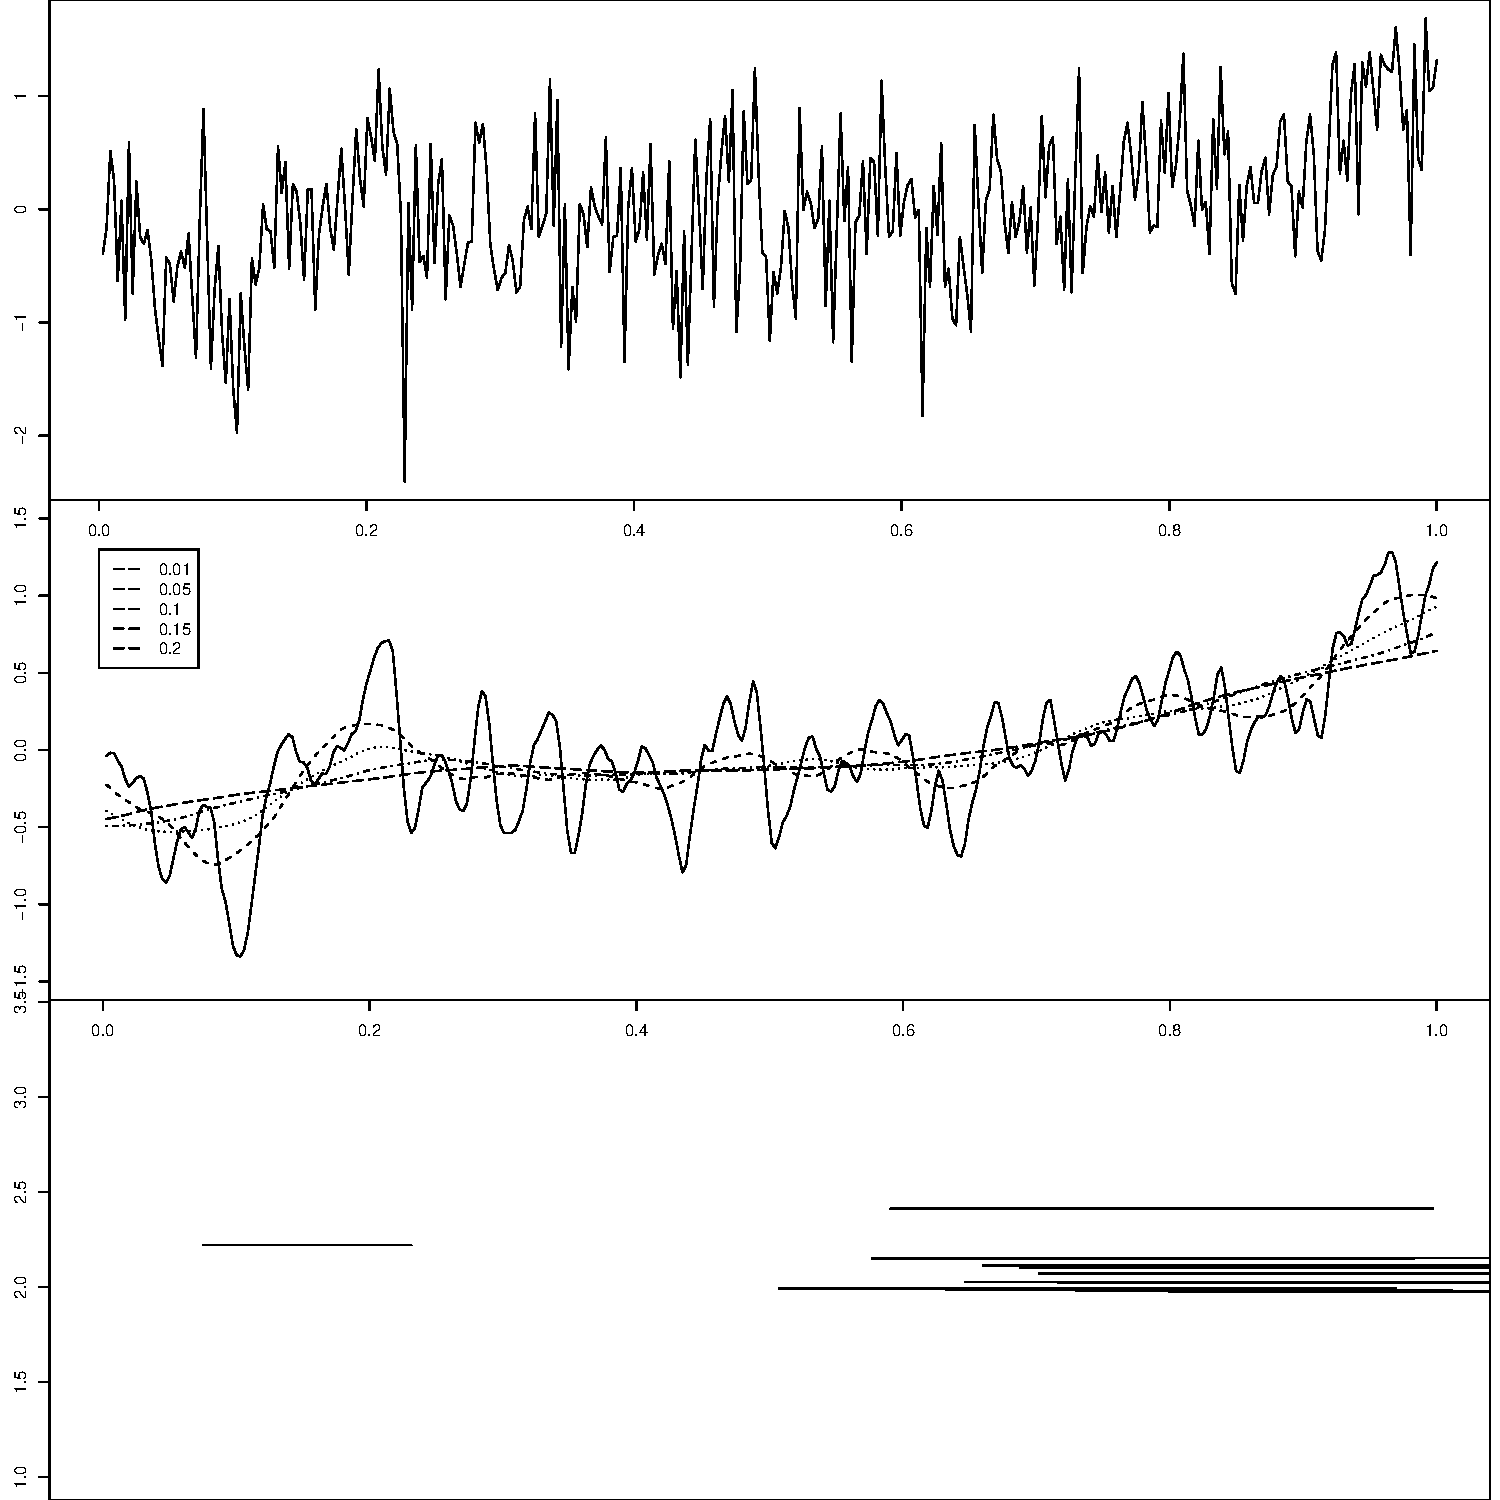
\includepdf[pages=-,pagecommand={},width=\textwidth]{Coding/Output/threegraphics.pdf}
\caption{Yearly temperature data for England\label{yearly_data}}
\end{figure}


\newpage
\section*{Appendix}

\def\theequation{A.\arabic{equation}}
\setcounter{equation}{0}
\allowdisplaybreaks[3]



In what follows, we prove the main theoretical results of the paper. Throughout the Appendix, the symbol $C$ denotes a universal real constant which may take a different value on each occurrence. We use the following notation: For $a,b \in \reals$, we write $a_+ = \max \{0,a\}$ and $a \vee b = \max\{a,b\}$. For any set $A$, the symbol $|A|$ denotes the cardinality of $A$. The notation $X \stackrel{\mathcal{D}}{=} Y$ means that the two random variables $X$ and $Y$ have the same distribution. Finally, $f_0(\cdot)$ and $F_0(\cdot)$ denote the density and distribution function of the standard Gaussian distribution, respectively.



\subsection*{Auxiliary results using strong approximation theory}


The main purpose of this section is to show that there is a version of the multiscale statistic $\widehat{\Phi}_T$ defined in \eqref{Phi-hat-statistic} which is close to a Gaussian statistic whose distribution is known. More specifically, we prove the following result. 
%
%
\begin{propA}\label{propA-strong-approx}
Under the conditions of Theorem \ref{theo-stat}, there exist statistics $\widetilde{\Phi}_T$ for $T = 1,2,\ldots$ with the following two properties: (i) $\widetilde{\Phi}_T$ has the same distribution as $\widehat{\Phi}_T$ for any $T$, and (ii)
\[ \big| \widetilde{\Phi}_T - \Phi_T \big| = o_p \Big( \frac{T^{1/q}}{\sqrt{T h_{\min}}} \Big), \]
where $\Phi_T$ is a Gaussian statistic as defined in \eqref{Phi-statistic}. 
\end{propA}
%
%
\begin{proof}[\textnormal{\textbf{Proof of Proposition \ref{propA-strong-approx}}}] 
For the proof, we draw on strong approximation theory for stationary processes $\{\varepsilon_t\}$ that fulfill the conditions \ref{C-err1}--\ref{C-err3}. By Theorem 2.1 and Corollary 2.1 in \cite{BerkesLiuWu2014}, the following strong approximation result holds true: On a richer probability space, there exists a standard Brownian motion $\mathbb{B}$ and a sequence $\{ \widetilde{\varepsilon}_t: 1 \le t \le T \}$ with $[\widetilde{\varepsilon}_1,\ldots,\widetilde{\varepsilon}_T] \stackrel{\mathcal{D}}{=} [\varepsilon_1,\ldots,\varepsilon_T]$ such that 
\begin{equation}\label{eq-strongapprox-dep}
\max_{1 \le t \le T} \Big| \sum\limits_{s=1}^t \widetilde{\varepsilon}_s - \sigma \mathbb{B}(t) \Big| = o\big( T^{1/q} \big) \quad \text{a.s.},  
\end{equation}
where $\sigma^2 = \sum_{k \in \integers} \cov(\varepsilon_0, \varepsilon_k)$ denotes the long-run error variance. To apply this result, we let 
\[ \widetilde{\Phi}_T = \max_{(u,h) \in \mathcal{G}_T} \Big\{ \Big|\frac{\widetilde{\phi}_T(u,h)}{\widetilde{\sigma}}\Big| - \lambda(h) \Big\}, \]
where $\widetilde{\phi}_T(u,h) = \sum\nolimits_{t=1}^T w_{t,T}(u,h) \widetilde{\varepsilon}_t$ and $\widetilde{\sigma}^2$ is the same estimator as $\widehat{\sigma}^2$ with $Y_t = m(t/T) + \varepsilon_t$ replaced by $\widetilde{Y}_t = m(t/T) + \widetilde{\varepsilon}_t$ for $1 \le t \le T$. In addition, we define
\begin{align*}
\Phi_T & = \max_{(u,h) \in \mathcal{G}_T} \Big\{ \Big|\frac{\phi_T(u,h)}{\sigma}\Big| - \lambda(h) \Big\} \\
\Phi_T^{*} & = \max_{(u,h) \in \mathcal{G}_T} \Big\{ \Big|\frac{\phi_T(u,h)}{\widetilde{\sigma}}\Big| - \lambda(h) \Big\} 
\end{align*}
with $\phi_T(u,h) = \sum\nolimits_{t=1}^T w_{t,T}(u,h) \sigma Z_t$ and $Z_t = \mathbb{B}(t) - \mathbb{B}(t-1)$. With this notation, we can write 
\begin{equation}\label{eq-strongapprox-bound1}
\big| \widetilde{\Phi}_T - \Phi_T \big| \le \big| \widetilde{\Phi}_T - \Phi_T^{*} \big| + \big| \Phi_T^{*} - \Phi_T \big| = \big| \widetilde{\Phi}_T - \Phi_T^{*} \big| + O_p \Big( \sqrt{\frac{\log T}{T}} \Big), 
\end{equation}
where the last equality follows by taking into account that the variables $Z_t$ are independent standard normal and $|\mathcal{G}_T| = O(T^\theta)$ for some large but fixed constant $\theta$. Straightforward calculations yield that 
\[ \big| \widetilde{\Phi}_T - \Phi_T^{*} \big| \le \widetilde{\sigma}^{-1} \max_{(u,h) \in \mathcal{G}_T} \big| \widetilde{\phi}_T(u,h) - \phi_T(u,h) \big|. \]
Using summation by parts,
%($\sum_{i=1}^n a_i b_i = \sum_{i=1}^{n-1} A_i (b_i - b_{i+1}) + A_n b_n$ with $A_j = \sum_{j=1}^i a_j$) 
we further obtain that 
\begin{align*}
\big| \widetilde{\phi}_T(u,h) - \phi_T(u,h) \big| 
 & \le W_T(u,h) \max_{1 \le t \le T} \Big| \sum\limits_{s=1}^t \widetilde{\varepsilon}_s - \sigma \sum\limits_{s=1}^t \big\{ \mathbb{B}(s) - \mathbb{B}(s-1) \big\} \Big| \\
 & = W_T(u,h) \max_{1 \le t \le T} \Big| \sum\limits_{s=1}^t \widetilde{\varepsilon}_s - \sigma \mathbb{B}(t) \Big|,
\end{align*}
where
\[ W_T(u,h) = \sum\limits_{t=1}^{T-1} |w_{t+1,T}(u,h) - w_{t,T}(u,h)| + |w_{T,T}(u,h)|. \]
Standard arguments show that $\max_{(u,h) \in \mathcal{G}_T} W_T(u,h) = O( 1/\sqrt{Th_{\min}} )$. Applying the strong approximation result \eqref{eq-strongapprox-dep}, we can thus infer that 
\begin{align}
\big| \widetilde{\Phi}_T - \Phi_T^{*} \big| 
 & \le \widetilde{\sigma}^{-1} \max_{(u,h) \in \mathcal{G}_T} \big| \widetilde{\phi}_T(u,h) - \phi_T(u,h) \big| \nonumber \\
 & \le \widetilde{\sigma}^{-1} \max_{(u,h) \in \mathcal{G}_T} W_T(u,h) \max_{1 \le t \le T} \Big| \sum\limits_{s=1}^t \widetilde{\varepsilon}_s - \sigma \mathbb{B}(t) \Big| 
 = o_p \Big( \frac{T^{1/q}}{\sqrt{Th_{\min}}} \Big). \label{eq-strongapprox-bound2}
\end{align}
Plugging \eqref{eq-strongapprox-bound2} into \eqref{eq-strongapprox-bound1} completes the proof.
\end{proof}



\subsection*{Auxiliary results using anti-concentration bounds}


In this section, we establish some properties of the Gaussian statistic $\Phi_T$ defined in \eqref{Phi-statistic}. We in particular show that $\Phi_T$ does not concentrate too strongly in small regions of the form $[x-\delta_T,x+\delta_T]$ with $\delta_T$ converging to zero.  
%
%
\enlargethispage{0.1cm}
\begin{propA}\label{propA-anticon}
Under the conditions of Theorem \ref{theo-stat}, it holds that 
\[ \sup_{x \in \reals} \pr \Big( | \Phi_T - x | \le \delta_T \Big) = o(1), \]
where $\delta_T = T^{1/q} / \sqrt{T h_{\min}}$.
\end{propA}
%
%
\begin{proof}[\textnormal{\textbf{Proof of Proposition \ref{propA-anticon}}}] 
The main technical tool for proving Proposition \ref{propA-anticon} are anti-concentration bounds for Gaussian random vectors. The following proposition slightly generalizes anti-concentration results derived in \cite{Chernozhukov2015}, in particular Theorem 3 therein. 
\begin{propA}\label{theo-anticon}
Let $(X_1,\ldots,X_p)^\top$ be a Gaussian random vector in $\reals^p$ with $\ex[X_j] = \mu_j$ and $\var(X_j) = \sigma_j^2 > 0$ for $1 \le j \le p$. Define $\overline{\mu} = \max_{1 \le j \le p} |\mu_j|$ and $a_p = \ex[ \max_{1 \le j \le p} (X_j-\mu_j)/\sigma_j ]$ as well as $\underline{\sigma} = \min_{1 \le j \le p} \sigma_j$ and $\overline{\sigma} = \max_{1 \le j \le p} \sigma_j$. For every $\delta > 0$, it holds that
\[ \sup_{x \in \reals} \pr \Big( \big| \max_{1 \le j \le p} X_j - x \big| \le \delta \Big) \le C \delta \big\{ \overline{\mu} + a_p + \sqrt{1 \vee \log(\underline{\sigma}/\delta)} \big\}, \]
where $C > 0$ depends only on $\underline{\sigma}$ and $\overline{\sigma}$. 
\end{propA} 
For the sake of completeness, the proof of Proposition \ref{theo-anticon} is provided at the end of the Appendix. To apply Proposition \ref{theo-anticon} to our setting at hand, we introduce the following notation: We write $x = (u,h)$ along with $\mathcal{G}_T = \{ x : x \in \mathcal{G}_T \} = \{x_1,\ldots,x_p\}$, where $p := |\mathcal{G}_T| \le O(T^\theta)$ for some large but fixed $\theta > 0$ by our assumptions. Moreover, for $j = 1,\ldots,p$, we set 
\[ X_{2j-1} = \frac{\phi_T(x_{j1},x_{j2})}{\sigma} - \lambda(x_{j2}) \]
and 
\[ X_{2j} = -\frac{\phi_T(x_{j1},x_{j2})}{\sigma} - \lambda(x_{j2}) \]
with $x_j = (x_{j1},x_{j2})$. This notation allows us to write
\[ \Phi_T = \max_{1 \le j \le 2p} X_j, \]
where $(X_1,\ldots,X_{2p})^\top$ is a Gaussian random vector with the following properties: (i) $\mu_j := \ex[X_j] = - \lambda(x_{j2})$ and thus $\overline{\mu} = \max_{1 \le j \le p} |\mu_j| \le C \sqrt{\log T}$, and (ii) $\var(X_j) = \sigma_j^2$ with $0 < \underline{\sigma} \le \sigma_j \le \overline{\sigma} < \infty$ for some fixed constants $\underline{\sigma}$, $\overline{\sigma}$ that are independent of $T$. Since the variables $(X_j - \mu_j)/\sigma_j$ are standard normal, it holds that $a_p \le \sqrt{2 \log (2p)} \le C \sqrt{\log T}$. With this notation at hand, we can apply Proposition \ref{theo-anticon} to obtain that 
\[ \sup_{x \in \reals} \pr \Big( \big| \Phi_T - x \big| \le \delta_T \Big) \le C \delta_T \Big[ \sqrt{\log T} + \sqrt{ \log(\underline{\sigma}/\delta_T) } \Big] = o(1) \]
with $\delta_T = T^{1/q} / \sqrt{T h_{\min}}$, which is the statement of Proposition \ref{propA-anticon}.
\end{proof}



\newpage
\subsection*{Proof of Theorem \ref{theo-stat}}


To prove Theorem \ref{theo-stat}, we make use of the two auxiliary results derived above. By Proposition \ref{propA-strong-approx}, there exist statistics $\widetilde{\Phi}_T$ for $T = 1,2,\ldots$ which are distributed as $\widehat{\Phi}_T$ for any $T \ge 1$ and which have the property that 
\begin{equation}\label{statement-propA-strong-approx}
\big| \widetilde{\Phi}_T - \Phi_T \big| = o_p \Big( \frac{T^{1/q}}{\sqrt{T h_{\min}}} \Big), 
\end{equation}
where $\Phi_T$ is a Gaussian statistic as defined in \eqref{Phi-statistic}. The approximation result \eqref{statement-propA-strong-approx} allows us to replace the multiscale statistic $\widehat{\Phi}_T$ by an identically distributed version $\widetilde{\Phi}_T$ which is close to the Gaussian statistic $\Phi_T$. In the next step, we show that  
\begin{equation}\label{eq-theo-stat-step2}
\sup_{x \in \reals} \big| \pr(\widetilde{\Phi}_T \le x) - \pr(\Phi_T \le x) \big| = o(1), 
\end{equation}
which immediately implies the statement of Theorem \ref{theo-stat}. For the proof of \eqref{eq-theo-stat-step2}, we use the following simple lemma: 
\begin{lemmaA}\label{lemma1-theo-stat}
Let $V_T$ and $W_T$ be real-valued random variables for $T = 1,2,\ldots$ such that $V_T - W_T = o_p(\delta_T)$ with $\delta_T = o(1)$. If 
\begin{equation}\label{eq-lemma1-cond}
\sup_{x \in \reals} \pr(|V_T - x| \le \delta_T) = o(1), 
\end{equation}
then 
\begin{equation}\label{eq-lemma1-statement}
\sup_{x \in \reals} \big| \pr(V_T \le x) - \pr(W_T \le x) \big| = o(1). 
\end{equation}
\end{lemmaA}
The statement of Lemma \ref{lemma1-theo-stat} can be summarized as follows: If $W_T$ can be approximated by $V_T$ in the sense that $V_T - W_T = o_p(\delta_T)$ and if $V_T$ does not concentrate too strongly in small regions of the form $[x - \delta_T,x+\delta_T]$ as assumed in \eqref{eq-lemma1-cond}, then the distribution of $W_T$ can be approximated by that of $V_T$ in the sense of \eqref{eq-lemma1-statement}.
\begin{proof}[\textnormal{\textbf{Proof of Lemma \ref{lemma1-theo-stat}}}] 
It holds that 
\begin{align*}
 & \big| \pr(V_T \le x) - \pr(W_T \le x) \big| \\
 & = \big| \ex \big[ 1(V_T \le x) - 1(W_T \le x) \big] \big| \\
 & \le \big| \ex \big[ \big\{ 1(V_T \le x) - 1(W_T \le x) \big\} 1(|V_T - W_T| \le \delta_T) \big] + \ex \big[ 1(|V_T - W_T| > \delta_T) \big] \big| \\
 & \le \ex \big[ 1(|V_T - x| \le \delta_T, |V_T - W_T| \le \delta_T) \big] + o(1) \\
 & \le \pr (|V_T - x| \le \delta_T) + o(1). \qedhere
\end{align*}
\end{proof}
We now apply this lemma with $V_T = \Phi_T$, $W_T = \widetilde{\Phi}_T$ and $\delta_T = T^{1/q} / \sqrt{T h_{\min}}$: From \eqref{statement-propA-strong-approx}, we already know that $\widetilde{\Phi}_T - \Phi_T = o_p(\delta_T)$. Moreover, by Proposition \ref{propA-anticon}, it holds that 
\begin{equation}\label{statement-propA-anticon}
\sup_{x \in \reals} \pr \Big( | \Phi_T - x | \le \delta_T \Big) = o(1). 
\end{equation}
Note that with the help of Theorem 2.1 in \cite{DuembgenSpokoiny2001}, we can further show that $\Phi_T = O_p(1)$. Together with \eqref{statement-propA-anticon}, this says that the Gaussian multiscale statistic $\Phi_T$ is asymptotically tight and does not concentrate too strongly in small regions of the form $[x - \delta_T,x + \delta_T]$. Putting everything together, we are now in a position to apply Lemma \ref{lemma1-theo-stat}, which in turn yields \eqref{eq-theo-stat-step2}. This completes the proof of Theorem \ref{theo-stat}. 



\subsection*{Proof of Proposition \ref{prop-test-3}}

 
The statement of Proposition \ref{prop-test-3} is a consequence of the following observation: For all $(u,h) \in \mathcal{G}_T$ with 
\[ \Big|\frac{\widehat{\psi}_T(u,h) - \ex \widehat{\psi}_T(u,h)}{\widehat{\sigma}}\Big| - \lambda(h) \le q_T(\alpha) \quad \text{and} \quad \Big|\frac{\widehat{\psi}_T(u,h)}{\widehat{\sigma}}\Big| - \lambda(h) > q_T(\alpha), \]
it holds that $\ex[\widehat{\psi}_T(u,h)] \ne 0$, which in turn implies that $m(v) \ne 0$ for some $v \in I_{u,h}$. From this observation, we can infer the following: On the event 
\[ \big\{ \widehat{\Phi}_T \le q_T(\alpha) \big\} = \Big\{ \max_{(u,h) \in \mathcal{G}_T} \Big( \Big|\frac{\widehat{\psi}_T(u,h) - \ex \widehat{\psi}_T(u,h)}{\widehat{\sigma}}\Big| - \lambda(h) \Big) \le q_T(\alpha) \Big\}, \]
it holds that for all $(u,h) \in \mathcal{A}_T$, 
$m(v) \ne 0$ for some $v \in I_{u,h}$. Hence, we obtain that 
\[ \big\{ \widehat{\Phi}_T \le q_T(\alpha) \big\} \subseteq E_T. \]
As a result, we arrive at  
\[ \pr(E_T) \ge \pr \big(  \widehat{\Phi}_T \le q_T(\alpha) \big) = (1-\alpha) + o(1), \]
where the last equality holds by Theorem \ref{theo-stat}.



\subsection*{Proof of Proposition \ref{theo-anticon}}

 
The proof makes use of the following three lemmas, which correspond to Lemmas 5--7 in \cite{Chernozhukov2015}. 
\begin{lemmaA}\label{lemma1-anticon}
Let $(W_1,\ldots,W_p)^\top$ be a (not necessarily centred) Gaussian random vector in $\reals^p$ with $\var(W_j) = 1$ for all $1 \le j \le p$. Suppose that $\text{Corr}(W_j,W_k) < 1$ whenever $j \ne k$. Then the distribution of $\max_{1 \le j \le p} W_j$ is absolutely continuous with respect to Lebesgue measure and a version of the density is given by 
\[ f(x) = f_0(x) \sum\limits_{j=1}^p e^{\ex[W_j]x - \ex[W_j]^2/2} \, \pr \big(W_k \le x \text{ for all } k \ne j \, \big| \, W_j = x \big). \]
\end{lemmaA}
\begin{lemmaA}\label{lemma2-anticon}
Let $(W_0,W_1,\ldots,W_p)^\top$ be a (not necessarily centred) Gaussian random vector in $\reals^p$ with $\var(W_j) = 1$ for all $1 \le j \le p$. Suppose that $\ex[W_0] \ge 0$. Then the map 
\[ x \mapsto  e^{\ex[W_0]x - \ex[W_0]^2/2} \, \pr \big(W_j \le x \text{ for } 1 \le j \le p \, \big| \, W_0 = x \big) \]
is non-decreasing on $\reals$. 
\end{lemmaA}
\begin{lemmaA}\label{lemma3-anticon}
Let $(X_1,\ldots,X_p)^\top$ be a centred Gaussian random vector in $\reals^p$ with $\max_{1 \le j \le p} \ex[X_j^2] \le \sigma^2$ for some $\sigma^2 > 0$. Then for any $r > 0$, 
\[ \pr \Big( \max_{1 \le j \le p} X_j \ge \ex \Big[ \max_{1 \le j \le p} X_j \Big] + r \Big) \le e^{-r^2/(2\sigma^2)}. \]
\end{lemmaA} 
The proof of Lemmas \ref{lemma1-anticon} and \ref{lemma2-anticon} can be found in \cite{Chernozhukov2015}. Lemma \ref{lemma3-anticon} is a standard result on Gaussian concentration whose proof is given e.g.\ in \cite{Ledoux2001}; see in particular Theorem 7.1 therein. We now closely follow the arguments for the proof of Theorem 3 in \cite{Chernozhukov2015}. The proof splits up into three steps. 
\vspace{10pt}


\textit{Step 1.} Pick any $x \ge 0$ and set 
\[ W_j = \frac{X_j - x}{\sigma_j} + \frac{\overline{\mu} + x}{\underline{\sigma}}. \]
By construction, $\ex[W_j] \ge 0$ and $\var(W_j) = 1$. Defining $Z = \max_{1 \le j \le p} W_j$, we have  
\begin{align*}
\pr \Big( \Big| \max_{1 \le j \le p} X_j - x \Big| \le \delta \Big) 
 & \le \pr \Big( \Big| \max_{1 \le j \le p} \frac{X_j - x}{\sigma_j} \Big| \le \frac{\delta}{\underline{\sigma}} \Big) \\
 & \le \sup_{y \in \reals} \pr \Big( \Big| \max_{1 \le j \le p} \frac{X_j - x}{\sigma_j} + \frac{\overline{\mu} + x}{\underline{\sigma}} - y \Big| \le \frac{\delta}{\underline{\sigma}} \Big) \\
 & = \sup_{y \in \reals} \pr \Big( |Z - y| \le \frac{\delta}{\underline{\sigma}} \Big). 
\end{align*}
\vspace{1pt}


\textit{Step 2.} We now bound the density of $Z$. Without loss of generality, we assume that $\text{Corr}(W_j,W_k) < 1$ whenever $k \ne j$. The marginal distribution of $W_j$ is $\normal(\nu_j,1)$ with $\nu_j = \ex[W_j] = (\mu_j/\sigma_j + \overline{\mu}/{\underline{\sigma}}) + (x/\underline{\sigma} - x/\sigma_j) \ge 0$. Hence, by Lemmas \ref{lemma1-anticon} and \ref{lemma2-anticon}, the random variable $Z$ has a density of the form
\begin{equation}\label{eq-dens-Z}
f_p(z) = f_0(z) G_p(z), 
\end{equation}
where the map $z \mapsto G_p(z)$ is non-decreasing. Define $\overline{Z} = \max_{1 \le j \le p} (W_j - \ex[W_j])$ and set $\overline{z} = 2 \overline{\mu}/\underline{\sigma} + x(1/\underline{\sigma} - 1/\overline{\sigma})$ such that $\ex[W_j] \le \overline{z}$ for any $1 \le j \le p$. With these definitions at hand, we obtain that  
\begin{align*}
\int_z^{\infty} f_0(u)du \, G_p(z) & \le \int_z^{\infty} f_0(u) G_p(u) du = \pr(Z > z) \\ 
 & \le P(\overline{Z} > z - \overline{z}) \le \exp \Big( - \frac{(z - \overline{z} - \ex[\overline{Z}])^2_+}{2} \Big), 
\end{align*}
where the last inequality is due to Lemma \ref{lemma3-anticon}. Since $W_j - \ex[W_j] = (X_j - \mu_j)/\sigma_j$, it holds that 
\[ \ex[\overline{Z}] = \ex \Big[ \max_{1 \le j \le p} \Big\{ \frac{X_j-\mu_j}{\sigma_j} \Big\} \Big] =: a_p. \]
Hence, for every $z \in \reals$, 
\begin{equation}\label{eq-bound-Gp}
G_p(z) \le \frac{1}{1 - F_0(z)} \exp\Big( - \frac{(z - \overline{z} - a_p)_+^2}{2} \Big). 
\end{equation}
Mill's inequality states that for $z > 0$, 
\[ z \le \frac{f_0(z)}{1-F_0(z)} \le z \frac{1+z^2}{z^2}. \]
Since $(1+z^2)/z^2 \le 2$ for $z > 1$ and $f_0(z)/\{1-F_0(z)\} \le 1.53 \le 2$ for $z \in (-\infty,1)$, we can infer that
\[ \frac{f_0(z)}{1-F_0(z)} \le 2 (z \vee 1) \quad \text{for any } z \in \reals. \]
This together with \eqref{eq-dens-Z} and \eqref{eq-bound-Gp} yields that
\[ f_p(z) \le 2 (z \vee 1)  \exp\Big( - \frac{(z - \overline{z} - a_p)_+^2}{2} \Big) \quad \text{for any } z \in \reals. \]
\vspace{1pt}
 

\textit{Step 3.} By Step 2, for any $y \in \reals$ and $u > 0$, we have
\[ \pr( |Z - y| \le u) = \int_{y - u}^{y + u} f_p(z) dz \le 2u \max_{z \in [y-u,y+u]} f_p(z) \le 4u (\overline{z} + a_p + 1), \] 
where the last inequality follows from the fact that the map $z \mapsto z e^{-(z-a)^2/2}$ (with $a > 0$) is non-increasing on $[a+1,\infty)$. Combining this bound with Step 1, we get that for any $x \ge 0$ and $\delta > 0$, 
\begin{equation}\label{eq-bound1-Levy}
\pr \Big( \Big| \max_{1 \le j \le p} X_j - x \Big| \le \delta \Big) \le 4\delta \Big\{ \frac{2\overline{\mu}}{\underline{\sigma}} + |x| \Big(\frac{1}{\underline{\sigma}} - \frac{1}{\overline{\sigma}}\Big) + a_p + 1 \Big\} \big/ \underline{\sigma}. 
\end{equation} 
This inequality also holds for $x < 0$ by an analogous argument, and hence for all $x \in \reals$. 


Now let $0 < \delta \le \underline{\sigma}$. For any $|x| \le \delta + \overline{\mu} + \overline{\sigma}(a_p + \sqrt{2\log(\underline{\sigma}/\delta)})$, \eqref{eq-bound1-Levy} yields that 
\begin{align}
\pr \Big( \Big| \max_{1 \le j \le p} X_j - x \Big| \le \delta \Big) 
 & \le \frac{4 \delta}{\underline{\sigma}} \Big\{ \overline{\mu} \Big( \frac{3}{\underline{\sigma}} - \frac{1}{\overline{\sigma}} \Big) + \frac{\overline{\sigma}}{\underline{\sigma}} a_p + \Big( \frac{\overline{\sigma}}{\underline{\sigma}} - 1 \Big) \sqrt{2\log\Big(\frac{\underline{\sigma}}{\delta}\Big)} + 2 - \frac{\underline{\sigma}}{\overline{\sigma}} \Big\} \nonumber \\[0.2cm]
 & \le C \delta \big\{ \overline{\mu} + a_p + \sqrt{1 \vee \log(\underline{\sigma}/\delta)} \big\} \label{eq-bound2-Levy}
\end{align}
with a sufficiently large constant $C > 0$ that depends only on $\underline{\sigma}$ and $\overline{\sigma}$. For $|x| \ge \delta + \overline{\mu} + \overline{\sigma}(a_p + \sqrt{2\log(\underline{\sigma}/\delta)})$, we obtain that 
\begin{equation}\label{eq-bound3-Levy}
\pr \Big( \Big| \max_{1 \le j \le p} X_j - x \Big| \le \delta \Big) \le \frac{\delta}{\underline{\sigma}}, 
\end{equation}
which can be seen as follows: If $x > \delta + \overline{\mu}$, then $|\max_j X_j - x| \le \delta$ implies that $|x| - \delta \le \max_j X_j \le \max_j \{ X_j - \mu_j \} + \overline{\mu}$ and thus $\max_j \{ X_j - \mu_j \} \ge |x| - \delta - \overline{\mu}$. It thus holds that 
\begin{equation}\label{eq-bound3-Levy-prep1}
\pr \Big( \Big| \max_{1 \le j \le p} X_j - x \Big| \le \delta \Big) \le \pr \Big( \max_{1 \le j \le p} \big\{ X_j - \mu_j \} \ge |x| - \delta - \overline{\mu} \Big). 
\end{equation}
If $x < - (\delta + \overline{\mu})$, then $|\max_j X_j - x| \le \delta$ implies that $\max_j \{ X_j - \mu_j \} \le -|x| + \delta + \overline{\mu}$. Hence, in this case,
\begin{align}
\pr \Big( \Big| \max_{1 \le j \le p} X_j - x \Big| \le \delta \Big) 
 & \le \pr \Big( \max_{1 \le j \le p} \big\{ X_j - \mu_j \} \le -|x| + \delta + \overline{\mu} \Big) \nonumber \\
 & \le \pr \Big( \max_{1 \le j \le p} \big\{ X_j - \mu_j \} \ge |x| - \delta - \overline{\mu} \Big), \label{eq-bound3-Levy-prep2}
\end{align}
where the last inequality follows from the fact that for centred Gaussian random variables $Z_j$ and $z > 0$, $\pr(\max_j Z_j \le - z) \le \pr(Z_1 \le -z) = P(Z_1 \ge z) \le \pr(\max_j Z_j \ge z)$. With \eqref{eq-bound3-Levy-prep1} and \eqref{eq-bound3-Levy-prep2}, we obtain that for any $|x| \ge \delta + \overline{\mu} + \overline{\sigma}(a_p + \sqrt{2\log(\underline{\sigma}/\delta)})$,
\begin{align*} 
\pr \Big( & \Big| \max_{1 \le j \le p} X_j - x \Big| \le \delta \Big) \le \pr \Big( \max_{1 \le j \le p} \big\{ X_j - \mu_j \} \ge |x| - \delta - \overline{\mu} \Big) \\
 & \le \pr \Big( \max_{1 \le j \le p} \big\{ X_j - \mu_j \big\} \ge \ex \Big[ \max_{1 \le j \le p} \big\{ X_j-\mu_j \big\} \Big] + \overline{\sigma} \sqrt{2\log(\underline{\sigma}/\delta)} \Big) \le \frac{\delta}{\underline{\sigma}}, 
\end{align*}
the last inequality following from Lemma \ref{lemma3-anticon}. To sum up, we have established that for any $0 < \delta \le \underline{\sigma}$ and any $x \in \reals$, 
\begin{equation}\label{claim-prop-anticon}
\pr \Big( \Big| \max_{1 \le j \le p} X_j - x \Big| \le \delta \Big) \le C \delta \big\{ \overline{\mu} + a_p + \sqrt{1 \vee \log(\underline{\sigma}/\delta)} \big\} 
\end{equation}
with some constant $C > 0$ that does only depend on $\underline{\sigma}$ and $\overline{\sigma}$. For $\delta > \underline{\sigma}$, \eqref{claim-prop-anticon} trivially follows upon setting $C \ge 1/\underline{\sigma}$. This completes the proof. 





\subsection*{Proof of Theorem \ref{theo-stat-equality}}

As already mentioned in Section \ref{subsec-test-equality-theo}, the proof is done by applying Theorem \ref{theo-stat} to our setting. More fomally, it goes as follows.


 
\begin{propA}\label{prop1-theo-stat-equality}
Under the conditions of Theorem \ref{theo-stat-equality}, there exist statistics $\widetilde{\Phi}_T$ for $T = 1,2,\ldots$ with the following two properties: (i) $\widetilde{\Phi}_T$ has the same distribution as $\widehat{\Phi}_T$ for any $T$, and (ii)
\[ \big| \widetilde{\Phi}_T - \Phi_T^* \big| = o_p \Big( \frac{T^{1/q}}{\sqrt{T h_{\min}}} \Big), \]
where $\Phi_T^*$ is a Gaussian statistic as defined in Section \ref{subsec-test-equality-theo}. 
\end{propA}
According to this result, we can replace the statistic $\widehat{\Phi}_T$ by an identically distributed version $\widetilde{\Phi}_T$ which is close to the Gaussian statistic $\Phi_T^*$. We defer the proof of Proposition \ref{prop1-theo-stat} until the arguments for Theorem \ref{theo-stat-equality} are completed. In the second main step of the proof, we show that 
\begin{equation}\label{eq-theo-stat-equality-step2}
\sup_{x \in \reals} \big| \pr(\widetilde{\Phi}_T \le x) - \pr(\Phi_T^* \le x) \big| = o(1), 
\end{equation}
which immediately implies the statement of Theorem \ref{theo-stat-equality}.

We now apply Lemma \ref{lemma1-theo-stat} with $V_T = \Phi^*_T$, $W_T = \widetilde{\Phi}_T$ and $\delta_T = T^{1/q} / \sqrt{T h_{\min}}$: Using L{\'e}vy's modulus of continuity, it can be shown that $\Phi_T^* = O_p(1)$. Moreover, from Proposition \ref{prop1-theo-stat-equality}, we already know that $\widetilde{\Phi}_T - \Phi_T^* = o_p(\delta_T)$. Finally, with the help of recent anti-concentration bounds for Gaussian random vectors, we can verify the following proposition.
\begin{propA}\label{prop2-theo-stat-equality}
Under the conditions of Theorem \ref{theo-stat-equality}, it holds that 
\[ \sup_{x \in \reals} \pr \Big( | \Phi_T^* - x | \le \delta_T \Big) = o(1). \]
\end{propA}
The proof of Proposition \ref{prop2-theo-stat-equality} is given below. According to it, the Gaussian multiscale statistic $\Phi_T^*$ does not concentrate too strongly in regions of the form $[x - \delta_T,x + \delta_T]$. Putting everything together, we are now in a position to apply Lemma \ref{lemma1-theo-stat}, which in turn yields \eqref{eq-theo-stat-step2}. This completes the proof of Theorem \ref{theo-stat-equality}. 



\subsubsection*{Proof of Proposition \ref{prop1-theo-stat-equality} -- strong approximation theory}


For the proof, we draw on strong approximation theory for stationary processes $\{\varepsilon_{it}\}$ for a fixed $i, 1\le i \le N$, that fulfill the conditions \ref{C-err1}--\ref{C-err3}. By Theorem 2.1 and Corollary 2.1 in \cite{BerkesLiuWu2014}, the following strong approximation result holds true: On a richer probability space, there exists a standard Brownian motion $\mathbb{B}_i$ and a sequence $\{ \widetilde{\varepsilon}_{it}: 1 \le t \le T \}$ with $[\widetilde{\varepsilon}_{i1},\ldots,\widetilde{\varepsilon}_{iT}] \stackrel{\mathcal{D}}{=} [\varepsilon_{i1},\ldots,\varepsilon_{iT}]$ such that 
\begin{equation}\label{eq-strongapprox-equality-dep}
\max_{1 \le t \le T} \Big| \sum\limits_{s=1}^t \widetilde{\varepsilon}_{is} - \sigma \mathbb{B}_i(t) \Big| = o\big( T^{1/q} \big) \quad \text{a.s.},  
\end{equation}
where $\sigma^2 = \sum_{k \in \integers} \ex[\varepsilon_{i0} \varepsilon_{ik}]$ denotes the long-run error variance.

To apply this result, we set
\begin{align*}
\widetilde{\Phi}_{ij,T} & = \max_{(u,h) \in \mathcal{G}_T} \Big\{ \Big|\frac{\widetilde{\phi}_{ij,T}(u,h)}{\sqrt{2}\widehat{\sigma}}\Big| - \lambda(h) \Big\},\\
\widetilde{\Phi}_T & = \max_{1\le i < j \le N} \widetilde{\Phi}_{ij,T}
\end{align*}
with $\widetilde{\phi}_{ij,T}(u,h) = \sum\nolimits_{t=1}^T w_{t,T}(u,h) (\widetilde{\varepsilon}_{it} - \widetilde{\varepsilon}_{jt})$ as well as 
\begin{align*}
\Phi_{ij,T}^* & = \max_{(u,h) \in \mathcal{G}_T} \Big\{ \Big|\frac{\phi_{ij,T}^*(u,h)}{\sqrt{2}\sigma}\Big| - \lambda(h) \Big\} \\
\Phi_T^* &= \max_{1\le i < j \le N} \Phi^*_{ij,T},\\
\Phi_{ij,T}^{**} & = \max_{(u,h) \in \mathcal{G}_T} \Big\{ \Big|\frac{\phi_{ij,T}^*(u,h)}{\sqrt{2}\widehat{\sigma}}\Big| - \lambda(h) \Big\},\\
\Phi_T^{**} &= \max_{1\le i < j \le N} \Phi^{**}_{ij,T}
\end{align*}
with $\phi_T^*(u,h) = \sum\nolimits_{t=1}^T w_{t,T}(u,h) (\sigma Z_{it} - \sigma Z_{jt})$ and $Z_{it} = \mathbb{B}_i(t) - \mathbb{B}_i(t-1)$. With this notation at hand, we get that 
\begin{equation}\label{eq-strongapprox-equality-bound1}
\big| \widetilde{\Phi}_T - \Phi_T^* \big| \le \big| \widetilde{\Phi}_T - \Phi_T^{**} \big| + \big| \Phi_T^{**} - \Phi_T^{*} \big| = \big| \widetilde{\Phi}_T - \Phi_T^{**} \big| + O_p \Big( \sqrt{\frac{\log T}{T}} \Big), 
\end{equation}
where the last equality holds due to 
% the fact that the variables $Z_t$ are independent standard normal and $|\mathcal{G}_T| = O(T^r)$ for some large but fixed constant $r$.
Moreover, straightforward calculations yield that 
\[ \big| \widetilde{\Phi}_T - \Phi_T^{**} \big| \le \widehat{\sigma}^{-1} \max_{1\le i<j \le N} \max_{(u,h) \in \mathcal{G}_T} \big| \widetilde{\phi}_{ij,T}(u,h) - \phi_{ij,T}^*(u,h) \big|. \]
Using summation by parts,
%($\sum_{i=1}^n a_i b_i = \sum_{i=1}^{n-1} A_i (b_i - b_{i+1}) + A_n b_n$ with $A_j = \sum_{j=1}^i a_j$) 
we obtain that 
\begin{align*}
\big| \widetilde{\phi}_T(u,h) - \phi_T^*(u,h) \big| 
 & \le \widehat{\sigma}^{-1} W_T(u,h) \max_{1 \le t \le T} \Big| \sum\limits_{s=1}^t \widetilde{\varepsilon}_s - \sigma \sum\limits_{s=1}^t \big\{ \mathbb{B}(s) - \mathbb{B}(s-1) \big\} \Big| \\
 & = \widehat{\sigma}^{-1} W_T(u,h) \max_{1 \le t \le T} \Big| \sum\limits_{s=1}^t \widetilde{\varepsilon}_s - \sigma \mathbb{B}(t) \Big|,
\end{align*}
where
\[ W_T(u,h) = \sum\limits_{t=1}^{T-1} |w_{t+1,T}(u,h) - w_{t,T}(u,h)| + |w_{T,T}(u,h)|. \]
Standard arguments show that $\max_{(u,h) \in \mathcal{G}_T} |W_T(u,h)| = O( 1/\sqrt{Th_{\min}} )$. Applying the strong approximation result \eqref{eq-strongapprox-equality-dep}, we can thus infer that 
\begin{equation}\label{eq-strongapprox-equality-bound2}
\big| \widetilde{\Phi}_T - \Phi_T^{**} \big| \le \widehat{\sigma}^{-1} \max_{1\le i<j \le N} \max_{(u,h) \in \mathcal{G}_T} \big| \widetilde{\phi}_{ij,T}(u,h) - \phi_{ij,T}^*(u,h) \big| = o_p \Big( \frac{T^{1/q}}{\sqrt{Th_{\min}}} \Big). 
\end{equation}
Plugging \eqref{eq-strongapprox-equality-bound2} into \eqref{eq-strongapprox-equality-bound1} completes the proof.



\enlargethispage{0.2cm}
%\subsection*{Proof of Proposition \ref{prop2-theo-stat-equality} -- anti-concentration bounds}
%
%
%The main technical tools for proving Proposition \ref{prop2-theo-stat} are anti-concentration bounds for Gaussian random vectors. The following proposition slightly generalizes anti-concentration results derived in \cite{Chernozhukov2015}, in particular Theorem 3 therein. 
%\begin{propA}\label{prop-anticon}
%Let $(X_1,\ldots,X_p)^\top$ be a Gaussian random vector in $\reals^p$ with $\ex[X_j] = \mu_j$ and $\var(X_j) = \sigma_j^2 > 0$ for $1 \le j \le p$. Define $\overline{\mu} = \max_{1 \le j \le p} |\mu_j|$ and $a_p = \ex[ \max_{1 \le j \le p} (X_j-\mu_j)/\sigma_j ]$ as well as $\underline{\sigma} = \min_{1 \le j \le p} \sigma_j$ and $\overline{\sigma} = \max_{1 \le j \le p} \sigma_j$. For every $\delta > 0$, it holds that
%\[ \sup_{x \in \reals} \pr \Big( \big| \max_{1 \le j \le p} X_j - x \big| \le \delta \Big) \le C \delta \big\{ \overline{\mu} + a_p + \sqrt{1 \vee \log(\underline{\sigma}/\delta)} \big\}, \]
%where $C > 0$ depends only on $\underline{\sigma}$ and $\overline{\sigma}$. 
%\end{propA} 
%To apply Proposition \ref{prop-anticon} to our setting at hand, we introduce the following notation: We write $x_j =(x_{j1},x_{j2}) = (u,h)$ along with $\{x_1,\ldots,x_p\} = \{ x : x \in \mathcal{G}_T \} = \mathcal{G}_T$, where $p := |\mathcal{G}_T| \le O(T^r)$ for some large but fixed $r > 0$ by our assumptions. Moreover, for $j = 1,\ldots,p$, we set 
%\[ X_{2j-1} = \frac{\phi_T^*(x_{j1},x_{j2})}{\sigma} - \lambda(x_{j2}) \quad \text{and} \quad X_{2j} = -\frac{\phi_T^*(x_{j1},x_{j2})}{\sigma} - \lambda(x_{j2}). \]
%This notation allows us to write
%\[ \Phi_T^* = \max_{1 \le j \le 2p} X_j, \]
%where $(X_1,\ldots,X_{2p})^\top$ is a Gaussian random vector with the following properties: (i) $\mu_j := \ex[X_j] = - \lambda(x_{j2})$ and thus $\overline{\mu} = \max_{1 \le j \le p} |\mu_j| \le C \sqrt{\log T}$, and (ii) $\var(X_j) = \sigma_j^2$ with $0 < \underline{\sigma} \le \sigma_j \le \overline{\sigma} < \infty$ for some fixed constants $\underline{\sigma}$, $\overline{\sigma}$ that are independent of $T$. Since the variables $(X_j - \mu_j)/\sigma_j$ are standard normal, it holds that $a_p \le \sqrt{2 \log (2p)} \le C \sqrt{\log T}$. With this notation at hand, we can apply Proposition \ref{prop-anticon} to obtain that 
%\[ \sup_{x \in \reals} \pr \Big( \big| \Phi_T^* - x \big| \le \delta_T \Big) \le C \delta_T \Big[ \sqrt{\log T} + \sqrt{ \log(\underline{\sigma}/\delta_T) } \Big] = o(1) \]
%with $\delta_T = T^{1/q} / \sqrt{T h_{\min}}$, which is the statement of Proposition \ref{prop2-theo-stat}.
%
%
%\begin{proof}[\textnormal{\textbf{Proof of Proposition \ref{prop-anticon}}}] 
%The proof makes use of the following three lemmas, which correspond to Lemmas 5--7 in \cite{Chernozhukov2015}. 
%\begin{lemmaA}\label{lemma1-anticon}
%Let $(W_1,\ldots,W_p)^\top$ be a (not necessarily centred) Gaussian random vector in $\reals^p$ with $\var(W_j) = 1$ for all $1 \le j \le p$. Suppose that $\text{Corr}(W_j,W_k) < 1$ whenever $j \ne k$. Then the distribution of $\max_{1 \le j \le p} W_j$ is absolutely continuous with respect to Lebesgue measure and a version of the density is given by 
%\[ f(x) = f_0(x) \sum\limits_{j=1}^p e^{\ex[W_j]x - (\ex[W_j])^2/2} \, \pr \big(W_k \le x \text{ for all } k \ne j \, \big| \, W_j = x \big). \]
%\end{lemmaA}
%\begin{lemmaA}\label{lemma2-anticon}
%Let $(W_0,W_1,\ldots,W_p)^\top$ be a (not necessarily centred) Gaussian random vector in $\reals^p$ with $\var(W_j) = 1$ for all $0 \le j \le p$. Suppose that $\ex[W_0] \ge 0$. Then the map 
%\[ x \mapsto  e^{\ex[W_0]x - (\ex[W_0])^2/2} \, \pr \big(W_j \le x \text{ for } 1 \le j \le p \, \big| \, W_0 = x \big) \]
%is non-decreasing on $\reals$. 
%\end{lemmaA}
%\begin{lemmaA}\label{lemma3-anticon}
%Let $(X_1,\ldots,X_p)^\top$ be a centred Gaussian random vector in $\reals^p$ with $\max_{1 \le j \le p} \ex[X_j^2] \le \sigma^2$ for some $\sigma^2 > 0$. Then for any $r > 0$, 
%\[ \pr \Big( \max_{1 \le j \le p} X_j \ge \ex \Big[ \max_{1 \le j \le p} X_j \Big] + r \Big) \le e^{-r^2/(2\sigma^2)}. \]
%\end{lemmaA} 
%The proofs of Lemmas \ref{lemma1-anticon} and \ref{lemma2-anticon} can be found in \cite{Chernozhukov2015}. Lemma \ref{lemma3-anticon} is a standard result on Gaussian concentration which proof is given e.g.\ in \cite{Ledoux2001}; see in particular Theorem 7.1 therein.
%
%We now closely follow the arguments for the proof of Theorem 3 in \cite{Chernozhukov2015}. The proof splits up into three steps. 
%\vspace{10pt}
%
%
%\textit{Step 1.} Pick any $x \ge 0$ and set 
%\[ W_j = \frac{X_j - x}{\sigma_j} + \frac{\overline{\mu} + x}{\underline{\sigma}}. \]
%By construction, $\ex[W_j] \ge 0$ and $\var(W_j) = 1$. Defining $Z = \max_{1 \le j \le p} W_j$, we have  
%\begin{align*}
%\pr \Big( \Big| \max_{1 \le j \le p} X_j - x \Big| \le \delta \Big) 
% & \le \pr \Big( \Big| \max_{1 \le j \le p} \frac{X_j - x}{\sigma_j} \Big| \le \frac{\delta}{\underline{\sigma}} \Big) \\
% & \le \sup_{y \in \reals} \pr \Big( \Big| \max_{1 \le j \le p} \frac{X_j - x}{\sigma_j} + \frac{\overline{\mu} + x}{\underline{\sigma}} - y \Big| \le \frac{\delta}{\underline{\sigma}} \Big) \\
% & = \sup_{y \in \reals} \pr \Big( |Z - y| \le \frac{\delta}{\underline{\sigma}} \Big). 
%\end{align*}
%\vspace{1pt}
%
%
%\textit{Step 2.} We now bound the density of $Z$. Without loss of generality, we assume that $\text{Corr}(W_j,W_k) < 1$ whenever $k \ne j$. The marginal distribution of $W_j$ is $\normal(\nu_j,1)$ with $\nu_j = \ex[W_j] = (\mu_j/\sigma_j + \overline{\mu}/{\underline{\sigma}}) + (x/\underline{\sigma} - x/\sigma_j) \ge 0$. Hence, by Lemmas \ref{lemma1-anticon} and \ref{lemma2-anticon}, the random variable $Z$ has a density of the form
%\begin{equation}\label{eq-dens-Z}
%f_p(z) = f_0(z) G_p(z), 
%\end{equation}
%where the map $z \mapsto G_p(z)$ is non-decreasing. Define $\overline{Z} = \max_{1 \le j \le p} (W_j - \ex[W_j])$ and set $\overline{z} = 2 \overline{\mu}/\underline{\sigma} + x(1/\underline{\sigma} - 1/\overline{\sigma})$ such that $\ex[W_j] \le \overline{z}$ for any $1 \le j \le p$. With these definitions at hand, we obtain that  
%\begin{align*}
%\int_z^{\infty} f_0(u)du \, G_p(z) & \le \int_z^{\infty} f_0(u) G_p(u) du = \pr(Z > z) \\ 
% & \le P(\overline{Z} > z - \overline{z}) \le \exp \Big( - \frac{(z - \overline{z} - \ex[\overline{Z}])^2_+}{2} \Big), 
%\end{align*}
%where the last inequality is due to Lemma \ref{lemma3-anticon}. Since $W_j - \ex[W_j] = (X_j - \mu_j)/\sigma_j$, it holds that 
%\[ \ex[\overline{Z}] = \ex \Big[ \max_{1 \le j \le p} \Big\{ \frac{X_j-\mu_j}{\sigma_j} \Big\} \Big] =: a_p. \]
%Hence, for every $z \in \reals$, 
%\begin{equation}\label{eq-bound-Gp}
%G_p(z) \le \frac{1}{1 - F_0(z)} \exp\Big( - \frac{(z - \overline{z} - a_p)_+^2}{2} \Big). 
%\end{equation}
%Mill's inequality states that for $z > 0$, 
%\[ z \le \frac{f_0(z)}{1-F_0(z)} \le z \frac{1+z^2}{z^2}. \]
%Since $(1+z^2)/z^2 \le 2$ for $z > 1$ and $f_0(z)/\{1-F_0(z)\} \le 1.53 \le 2$ for $z \in (-\infty,1)$, we can infer that
%\[ \frac{f_0(z)}{1-F_0(z)} \le 2 (z \vee 1) \quad \text{for any } z \in \reals. \]
%This together with \eqref{eq-dens-Z} and \eqref{eq-bound-Gp} yields that
%\[ f_p(z) \le 2 (z \vee 1)  \exp\Big( - \frac{(z - \overline{z} - a_p)_+^2}{2} \Big) \quad \text{for any } z \in \reals. \]
%\vspace{1pt}
% 
%
%\textit{Step 3.} By Step 2, for any $y \in \reals$ and $u > 0$, we have
%\[ \pr( |Z - y| \le u) = \int_{y - u}^{y + u} f_p(z) dz \le 2u \max_{z \in [y-u,y+u]} f_p(z) \le 4u (\overline{z} + a_p + 1), \] 
%where the last inequality follows from the fact that the map $z \mapsto z e^{-(z-a)^2/2}$ (with $a > 0$) is non-increasing on $[a+1,\infty)$. Combining this bound with Step 1, we get that for any $x \ge 0$ and $\delta > 0$, 
%\begin{equation}\label{eq-bound1-Levy}
%\pr \Big( \Big| \max_{1 \le j \le p} X_j - x \Big| \le \delta \Big) \le 4\delta \Big\{ \frac{2\overline{\mu}}{\underline{\sigma}} + |x| \Big(\frac{1}{\underline{\sigma}} - \frac{1}{\overline{\sigma}}\Big) + a_p + 1 \Big\} \big/ \underline{\sigma}. 
%\end{equation} 
%This inequality also holds for $x < 0$ by the analogous argument, and hence for all $x \in \reals$. 
%
%
%Now let $0 < \delta \le \underline{\sigma}$. For any $|x| \le \delta + \overline{\mu} + \overline{\sigma}(a_p + \sqrt{2\log(\underline{\sigma}/\delta)})$, \eqref{eq-bound1-Levy} yields that 
%\begin{align}
%\pr \Big( \Big| \max_{1 \le j \le p} X_j - x \Big| \le \delta \Big) 
% & \le \frac{4 \delta}{\underline{\sigma}} \Big\{ \overline{\mu} \Big( \frac{3}{\underline{\sigma}} - \frac{1}{\overline{\sigma}} \Big) + \frac{\overline{\sigma}}{\underline{\sigma}} a_p + \Big( \frac{\overline{\sigma}}{\underline{\sigma}} - 1 \Big) \sqrt{2\log\Big(\frac{\underline{\sigma}}{\delta}\Big)} + 2 - \frac{\underline{\sigma}}{\overline{\sigma}} \Big\} \nonumber \\[0.2cm]
% & \le C \delta \big\{ \overline{\mu} + a_p + \sqrt{1 \vee \log(\underline{\sigma}/\delta)} \big\} \label{eq-bound2-Levy}
%\end{align}
%with a sufficiently large constant $C > 0$ that depends only on $\underline{\sigma}$ and $\overline{\sigma}$. For \linebreak  $|x| \ge \delta + \overline{\mu} + \overline{\sigma}(a_p + \sqrt{2\log(\underline{\sigma}/\delta)})$, we obtain that 
%\begin{equation}\label{eq-bound3-Levy}
%\pr \Big( \Big| \max_{1 \le j \le p} X_j - x \Big| \le \delta \Big) \le \frac{\delta}{\underline{\sigma}}, 
%\end{equation}
%which can be seen as follows: If $x > \delta + \overline{\mu}$, then $|\max_j X_j - x| \le \delta$ implies that $|x| - \delta \le \max_j X_j \le \max_j \{ X_j - \mu_j \} + \overline{\mu}$ and thus $\max_j \{ X_j - \mu_j \} \ge |x| - \delta - \overline{\mu}$. It thus holds that 
%\begin{equation}\label{eq-bound3-Levy-prep1}
%\pr \Big( \Big| \max_{1 \le j \le p} X_j - x \Big| \le \delta \Big) \le \pr \Big( \max_{1 \le j \le p} \big\{ X_j - \mu_j \} \ge |x| - \delta - \overline{\mu} \Big). 
%\end{equation}
%If $x < - (\delta + \overline{\mu})$, then $|\max_j X_j - x| \le \delta$ implies that $\max_j \{ X_j - \mu_j \} \le -|x| + \delta + \overline{\mu}$. Hence, in this case,
%\begin{align}
%\pr \Big( \Big| \max_{1 \le j \le p} X_j - x \Big| \le \delta \Big) 
% & \le \pr \Big( \max_{1 \le j \le p} \big\{ X_j - \mu_j \} \le -|x| + \delta + \overline{\mu} \Big) \nonumber \\
% & \le \pr \Big( \max_{1 \le j \le p} \big\{ X_j - \mu_j \} \ge |x| - \delta - \overline{\mu} \Big), \label{eq-bound3-Levy-prep2}
%\end{align}
%where the last inequality follows from the fact that for centred Gaussian random variables $Z_j$ and $\forall z > 0$, $\pr(\max_j Z_j \le - z) \le \pr(Z_1 \le -z) = P(Z_1 \ge z) \le \pr(\max_j Z_j \ge z)$. With \eqref{eq-bound3-Levy-prep1} and \eqref{eq-bound3-Levy-prep2}, we obtain that for any $|x| \ge \delta + \overline{\mu} + \overline{\sigma}(a_p + \sqrt{2\log(\underline{\sigma}/\delta)})$,
%\begin{align*} 
%\pr \Big( & \Big| \max_{1 \le j \le p} X_j - x \Big| \le \delta \Big) \le \pr \Big( \max_{1 \le j \le p} \big\{ X_j - \mu_j \} \ge |x| - \delta - \overline{\mu} \Big) \\
% & \le \pr \Big( \max_{1 \le j \le p} \big\{ X_j - \mu_j \big\} \ge \ex \Big[ \max_{1 \le j \le p} \big\{ X_j-\mu_j \big\} \Big] + \overline{\sigma} \sqrt{2\log(\underline{\sigma}/\delta)} \Big) \le \frac{\delta}{\underline{\sigma}}, 
%\end{align*}
%the last inequality following from Lemma \ref{lemma3-anticon}. To sum up, we have established that for any $0 < \delta \le \underline{\sigma}$ and any $x \in \reals$, 
%\begin{equation}\label{claim-prop-anticon}
%\pr \Big( \Big| \max_{1 \le j \le p} X_j - x \Big| \le \delta \Big) \le C \delta \big\{ \overline{\mu} + a_p + \sqrt{1 \vee \log(\underline{\sigma}/\delta)} \big\} 
%\end{equation}
%with some constant $C > 0$ that does only depend on $\underline{\sigma}$ and $\overline{\sigma}$. For $\delta > \underline{\sigma}$, \eqref{claim-prop-anticon} trivially follows upon setting $C \ge 1/\underline{\sigma}$. This completes the proof. 
%\end{proof}
%
%
%
%\subsection*{Proof of Corollary \ref{corollary-test-3}}
%
% 
%The statement of Corollary \ref{corollary-test-3} is a consequence of the following observation: For all $(u,h) \in \mathcal{G}_T$ with 
%\[ \Big|\frac{\widehat{\psi}_T(u,h) - \ex \widehat{\psi}_T(u,h)}{\widehat{\sigma}}\Big| - \lambda(h) \le q_T(\alpha) \quad \text{and} \quad \Big|\frac{\widehat{\psi}_T(u,h)}{\widehat{\sigma}}\Big| - \lambda(h) > q_T(\alpha), \]
%it holds that $\ex[\widehat{\psi}_T(u,h)] \ne 0$, which in turn implies that $m(v) \ne 0$ for some $v \in I_{u,h}$. From this observation, we can infer the following: On the event 
%\[ \big\{ \widehat{\Phi}_T \le q_T(\alpha) \big\} = \Big\{ \max_{(u,h) \in \mathcal{G}_T} \Big( \Big|\frac{\widehat{\psi}_T(u,h) - \ex \widehat{\psi}_T(u,h)}{\widehat{\sigma}}\Big| - \lambda(h) \Big) \le q_T(\alpha) \Big\}, \]
%it holds that for all $(u,h) \in \mathcal{A}_T$, 
%$m(v) \ne 0$ for some $v \in I_{u,h}$. Hence, we obtain that 
%\[ \big\{ \widehat{\Phi}_T \le q_T(\alpha) \big\} \subseteq E_T. \]
%As a result, we arrive at  
%\[ \pr(E_T) \ge \pr \big(  \widehat{\Phi}_T \le q_T(\alpha) \big) = (1-\alpha) + o(1), \]
%where the last equality holds by Theorem \ref{theo-stat}.

\newpage
\bibliographystyle{ims}
{\small
\setlength{\bibsep}{0.55em}
\bibliography{bibliography}}



\end{document}
